\documentclass[10pt, oneside]{article} 
\usepackage{amsmath, amsthm, amssymb, calrsfs, wasysym, verbatim, bbm, color, graphics, geometry, esint, float}


\geometry{tmargin=.75in, bmargin=.75in, lmargin=.75in, rmargin = .75in}  

\newcommand{\bbR}{\mathbb{R}}
\newcommand{\bbC}{\mathbb{C}}
\newcommand{\bbZ}{\mathbb{Z}}
\newcommand{\bbP}{\mathbb{P}}
\newcommand{\bbN}{\mathbb{N}}
\newcommand{\bbE}{\mathbb{E}}
\newcommand{\Var}{\text{Var}}
\newcommand{\bbQ}{\mathbb{Q}}
\newcommand{\Cdot}{\boldsymbol{\cdot}}
\newcommand{\scA}{\mathscr{A}}
\newcommand{\curl}{\text{curl}}

\theoremstyle{definition}
\newtheorem{exmp}{Example}[section]
\newtheorem{thm}{Theorem}
\newtheorem{defn}{Definition}
\newtheorem{prop}{Proposition}
\newtheorem{conv}{Convention}
\newtheorem{rem}{Remark}
\newtheorem{lem}{Lemma}
\newtheorem{cor}{Corollary}
% Copyright 2021 Paolo Adajar (padajar.com, paoloadajar@mit.edu)
% 
% Permission is hereby granted, free of charge, to any person obtaining a copy of this software and associated documentation files (the "Software"), to deal in the Software without restriction, including without limitation the rights to use, copy, modify, merge, publish, distribute, sublicense, and/or sell copies of the Software, and to permit persons to whom the Software is furnished to do so, subject to the following conditions:
%
% The above copyright notice and this permission notice shall be included in all copies or substantial portions of the Software.
% 
% THE SOFTWARE IS PROVIDED "AS IS", WITHOUT WARRANTY OF ANY KIND, EXPRESS OR IMPLIED, INCLUDING BUT NOT LIMITED TO THE WARRANTIES OF MERCHANTABILITY, FITNESS FOR A PARTICULAR PURPOSE AND NONINFRINGEMENT. IN NO EVENT SHALL THE AUTHORS OR COPYRIGHT HOLDERS BE LIABLE FOR ANY CLAIM, DAMAGES OR OTHER LIABILITY, WHETHER IN AN ACTION OF CONTRACT, TORT OR OTHERWISE, ARISING FROM, OUT OF OR IN CONNECTION WITH THE SOFTWARE OR THE USE OR OTHER DEALINGS IN THE SOFTWARE.

\usepackage{fullpage}
\usepackage{enumitem}
\usepackage{amsfonts, amssymb, amsmath,amsthm}
\usepackage{mathtools}
\usepackage[pdftex, pdfauthor={\name}, pdftitle={\classnum~\assignment}]{hyperref}
\usepackage[dvipsnames]{xcolor}
\usepackage{bbm}
\usepackage{graphicx}
\usepackage{mathrsfs}
\usepackage{pdfpages}
\usepackage{tabularx}
\usepackage{pdflscape}
\usepackage{makecell}
\usepackage{booktabs}
\usepackage{natbib}
\usepackage{caption}
\usepackage{subcaption}
\usepackage{physics}
\usepackage[many]{tcolorbox}
\usepackage{version}
\usepackage{ifthen}
\usepackage{cancel}
\usepackage{listings}
\usepackage{courier}

\usepackage{tikz}
\usepackage{istgame}

\hypersetup{
	colorlinks=true,
	linkcolor=blue,
	filecolor=magenta,
	urlcolor=blue,
}

\setlength{\parindent}{0mm}
\setlength{\parskip}{2mm}

\setlist[enumerate]{label=({\alph*})}
\setlist[enumerate, 2]{label=({\roman*})}

\allowdisplaybreaks[1]

\newcommand{\psetheader}{
	\ifthenelse{\isundefined{\collaborators}}{
		\begin{center}
			{\setlength{\parindent}{0cm} \setlength{\parskip}{0mm}
				
				{\textbf{\classnum~\semester:~\assignment} \hfill \name}
				
				\subject \hfill \href{mailto:\email}{\tt \email}
				
				Instructor(s):~\instructors \hfill Due Date:~\duedate	
				
				\hrulefill}
		\end{center}
	}{
		\begin{center}
			{\setlength{\parindent}{0cm} \setlength{\parskip}{0mm}
				
				{\textbf{\classnum~\semester:~\assignment} \hfill \name\footnote{Collaborator(s): \collaborators}}
				
				\subject \hfill \href{mailto:\email}{\tt \email}
				
				Instructor(s):~\instructors \hfill Due Date:~\duedate	
				
				\hrulefill}
		\end{center}
	}
}

\renewcommand{\thepage}{\classnum~\assignment \hfill \arabic{page}}

\makeatletter
\def\points{\@ifnextchar[{\@with}{\@without}}
\def\@with[#1]#2{{\ifthenelse{\equal{#2}{1}}{{[1 point, #1]}}{{[#2 points, #1]}}}}
\def\@without#1{\ifthenelse{\equal{#1}{1}}{{[1 point]}}{{[#1 points]}}}
\makeatother

\newtheoremstyle{theorem-custom}%
{}{}%
{}{}%
{\itshape}{.}%
{ }%
{\thmname{#1}\thmnumber{ #2}\thmnote{ (#3)}}

\theoremstyle{theorem-custom}

\newtheorem{theorem}{Theorem}
\newtheorem{lemma}[theorem]{Lemma}
\newtheorem{example}[theorem]{Example}

\newenvironment{problem}[1]{\color{black} #1}{}

\newenvironment{solution}{%
	\leavevmode\begin{tcolorbox}[breakable, colback=green!5!white,colframe=green!75!black, enhanced jigsaw] \proof[\scshape Solution:] \setlength{\parskip}{2mm}%
	}{\renewcommand{\qedsymbol}{$\blacksquare$} \endproof \end{tcolorbox}}

\newenvironment{reflection}{\begin{tcolorbox}[breakable, colback=black!8!white,colframe=black!60!white, enhanced jigsaw, parbox = false]\textsc{Reflections:}}{\end{tcolorbox}}

\newcommand{\qedh}{\renewcommand{\qedsymbol}{$\blacksquare$}\qedhere}

\definecolor{mygreen}{rgb}{0,0.6,0}
\definecolor{mygray}{rgb}{0.5,0.5,0.5}
\definecolor{mymauve}{rgb}{0.58,0,0.82}

% from https://github.com/satejsoman/stata-lstlisting
% language definition
\lstdefinelanguage{Stata}{
	% System commands
	morekeywords=[1]{regress, reg, summarize, sum, display, di, generate, gen, bysort, use, import, delimited, predict, quietly, probit, margins, test},
	% Reserved words
	morekeywords=[2]{aggregate, array, boolean, break, byte, case, catch, class, colvector, complex, const, continue, default, delegate, delete, do, double, else, eltypedef, end, enum, explicit, export, external, float, for, friend, function, global, goto, if, inline, int, local, long, mata, matrix, namespace, new, numeric, NULL, operator, orgtypedef, pointer, polymorphic, pragma, private, protected, public, quad, real, return, rowvector, scalar, short, signed, static, strL, string, struct, super, switch, template, this, throw, transmorphic, try, typedef, typename, union, unsigned, using, vector, version, virtual, void, volatile, while,},
	% Keywords
	morekeywords=[3]{forvalues, foreach, set},
	% Date and time functions
	morekeywords=[4]{bofd, Cdhms, Chms, Clock, clock, Cmdyhms, Cofc, cofC, Cofd, cofd, daily, date, day, dhms, dofb, dofC, dofc, dofh, dofm, dofq, dofw, dofy, dow, doy, halfyear, halfyearly, hh, hhC, hms, hofd, hours, mdy, mdyhms, minutes, mm, mmC, mofd, month, monthly, msofhours, msofminutes, msofseconds, qofd, quarter, quarterly, seconds, ss, ssC, tC, tc, td, th, tm, tq, tw, week, weekly, wofd, year, yearly, yh, ym, yofd, yq, yw,},
	% Mathematical functions
	morekeywords=[5]{abs, ceil, cloglog, comb, digamma, exp, expm1, floor, int, invcloglog, invlogit, ln, ln1m, ln, ln1p, ln, lnfactorial, lngamma, log, log10, log1m, log1p, logit, max, min, mod, reldif, round, sign, sqrt, sum, trigamma, trunc,},
	% Matrix functions
	morekeywords=[6]{cholesky, coleqnumb, colnfreeparms, colnumb, colsof, corr, det, diag, diag0cnt, el, get, hadamard, I, inv, invsym, issymmetric, J, matmissing, matuniform, mreldif, nullmat, roweqnumb, rownfreeparms, rownumb, rowsof, sweep, trace, vec, vecdiag, },
	% Programming functions
	morekeywords=[7]{autocode, byteorder, c, _caller, chop, abs, clip, cond, e, fileexists, fileread, filereaderror, filewrite, float, fmtwidth, has_eprop, inlist, inrange, irecode, matrix, maxbyte, maxdouble, maxfloat, maxint, maxlong, mi, minbyte, mindouble, minfloat, minint, minlong, missing, r, recode, replay, return, s, scalar, smallestdouble,},
	% Random-number functions
	morekeywords=[8]{rbeta, rbinomial, rcauchy, rchi2, rexponential, rgamma, rhypergeometric, rigaussian, rlaplace, rlogistic, rnbinomial, rnormal, rpoisson, rt, runiform, runiformint, rweibull, rweibullph,},
	% Selecting time-span functions
	morekeywords=[9]{tin, twithin,},
	% Statistical functions
	morekeywords=[10]{betaden, binomial, binomialp, binomialtail, binormal, cauchy, cauchyden, cauchytail, chi2, chi2den, chi2tail, dgammapda, dgammapdada, dgammapdadx, dgammapdx, dgammapdxdx, dunnettprob, exponential, exponentialden, exponentialtail, F, Fden, Ftail, gammaden, gammap, gammaptail, hypergeometric, hypergeometricp, ibeta, ibetatail, igaussian, igaussianden, igaussiantail, invbinomial, invbinomialtail, invcauchy, invcauchytail, invchi2, invchi2tail, invdunnettprob, invexponential, invexponentialtail, invF, invFtail, invgammap, invgammaptail, invibeta, invibetatail, invigaussian, invigaussiantail, invlaplace, invlaplacetail, invlogistic, invlogistictail, invnbinomial, invnbinomialtail, invnchi2, invnF, invnFtail, invnibeta, invnormal, invnt, invnttail, invpoisson, invpoissontail, invt, invttail, invtukeyprob, invweibull, invweibullph, invweibullphtail, invweibulltail, laplace, laplaceden, laplacetail, lncauchyden, lnigammaden, lnigaussianden, lniwishartden, lnlaplaceden, lnmvnormalden, lnnormal, lnnormalden, lnwishartden, logistic, logisticden, logistictail, nbetaden, nbinomial, nbinomialp, nbinomialtail, nchi2, nchi2den, nchi2tail, nF, nFden, nFtail, nibeta, normal, normalden, npnchi2, npnF, npnt, nt, ntden, nttail, poisson, poissonp, poissontail, t, tden, ttail, tukeyprob, weibull, weibullden, weibullph, weibullphden, weibullphtail, weibulltail,},
	% String functions 
	morekeywords=[11]{abbrev, char, collatorlocale, collatorversion, indexnot, plural, plural, real, regexm, regexr, regexs, soundex, soundex_nara, strcat, strdup, string, strofreal, string, strofreal, stritrim, strlen, strlower, strltrim, strmatch, strofreal, strofreal, strpos, strproper, strreverse, strrpos, strrtrim, strtoname, strtrim, strupper, subinstr, subinword, substr, tobytes, uchar, udstrlen, udsubstr, uisdigit, uisletter, ustrcompare, ustrcompareex, ustrfix, ustrfrom, ustrinvalidcnt, ustrleft, ustrlen, ustrlower, ustrltrim, ustrnormalize, ustrpos, ustrregexm, ustrregexra, ustrregexrf, ustrregexs, ustrreverse, ustrright, ustrrpos, ustrrtrim, ustrsortkey, ustrsortkeyex, ustrtitle, ustrto, ustrtohex, ustrtoname, ustrtrim, ustrunescape, ustrupper, ustrword, ustrwordcount, usubinstr, usubstr, word, wordbreaklocale, worcount,},
	% Trig functions
	morekeywords=[12]{acos, acosh, asin, asinh, atan, atanh, cos, cosh, sin, sinh, tan, tanh,},
	morecomment=[l]{//},
	% morecomment=[l]{*},  // `*` maybe used as multiply operator. So use `//` as line comment.
	morecomment=[s]{/*}{*/},
	% The following is used by macros, like `lags'.
	morestring=[b]{`}{'},
	% morestring=[d]{'},
	morestring=[b]",
	morestring=[d]",
	% morestring=[d]{\\`},
	% morestring=[b]{'},
	sensitive=true,
}

\lstset{ 
	backgroundcolor=\color{white},   % choose the background color; you must add \usepackage{color} or \usepackage{xcolor}; should come as last argument
	basicstyle=\footnotesize\ttfamily,        % the size of the fonts that are used for the code
	breakatwhitespace=false,         % sets if automatic breaks should only happen at whitespace
	breaklines=true,                 % sets automatic line breaking
	captionpos=b,                    % sets the caption-position to bottom
	commentstyle=\color{mygreen},    % comment style
	deletekeywords={...},            % if you want to delete keywords from the given language
	escapeinside={\%*}{*)},          % if you want to add LaTeX within your code
	extendedchars=true,              % lets you use non-ASCII characters; for 8-bits encodings only, does not work with UTF-8
	firstnumber=0,                % start line enumeration with line 1000
	frame=single,	                   % adds a frame around the code
	keepspaces=true,                 % keeps spaces in text, useful for keeping indentation of code (possibly needs columns=flexible)
	keywordstyle=\color{blue},       % keyword style
	language=Octave,                 % the language of the code
	morekeywords={*,...},            % if you want to add more keywords to the set
	numbers=left,                    % where to put the line-numbers; possible values are (none, left, right)
	numbersep=5pt,                   % how far the line-numbers are from the code
	numberstyle=\tiny\color{mygray}, % the style that is used for the line-numbers
	rulecolor=\color{black},         % if not set, the frame-color may be changed on line-breaks within not-black text (e.g. comments (green here))
	showspaces=false,                % show spaces everywhere adding particular underscores; it overrides 'showstringspaces'
	showstringspaces=false,          % underline spaces within strings only
	showtabs=false,                  % show tabs within strings adding particular underscores
	stepnumber=2,                    % the step between two line-numbers. If it's 1, each line will be numbered
	stringstyle=\color{mymauve},     % string literal style
	tabsize=2,	                   % sets default tabsize to 2 spaces
%	title=\lstname,                   % show the filename of files included with \lstinputlisting; also try caption instead of title
	xleftmargin=0.25cm
}



\title{UChicago Markov Chains, Martingales, and Brownian Motion Analysis Notes: 23500}
\author{Notes by Agustín Esteva, Lectures by Stephen Yearwood, Books by }
\date{Academic Year 2024-2025}

\begin{document}

\maketitle
\tableofcontents

\vspace{.25in}


\newpage
\section{Lectures}

\subsection{Monday, Mar 24: Markov Processes: Basic Definitions and Examples}
He is from Trinidad and Tobago. 
\begin{defn}
    A \textbf{stochastic process}  is a collection of random variables $\{X_t\}_{t \in T}$ indexed by time, where each $X_t$ takes values in $S$
\end{defn}
We call $S$ our \textit{state space}. In discrete time, it should be obvious that $T = \bbN_0^*$ (where $\bbN_0^*$ is when on goscale the naturals by a constant) and $T = [0, \bbR)$ in continuous time. We say that $S$ is a discrete space if it is countable and continuous if it is $\bbR^d.$
\begin{rem}
    In order to characterize the distribution of $\{X_n\},$ we must specify $\mathbb{P}\{X_0 = S_0, \dots, X_n = S_n\}$ for all $n \in \bbN$ and for all $S_0, \dots, S_n \in S.$ It is much easier work with conditional probability. We will see that with Markov Chains, the Markov Property guarantees that we only need to worry about the distribution of $X_{n-1}$ to figure out $X_n.$
\end{rem}
\begin{defn}
    If $E,F$ are events with $\mathbb{P}\{F\} >0,$ then the \textbf{conditional probability} of $E$ given $F$ is 
    \[\mathbb{P}(E | F) = \frac{\mathbb{P}(E \cap F)}{\mathbb{P}(F)}\]
\end{defn}
\begin{prop}
    (Law of Total Probability) Recall that if $(B_n) \in S$ is a sequence of mutually exclusive and exhaustive events, then 
    \[P(A) = \sum_{n=1}^\infty P(A \cap B_n) = \sum_{n=1}^\infty P(A \mid B_n)P(B_n)\]
\end{prop}

\begin{defn}
    A stochastic process is called a \textbf{Markov Chain} if for all $n \in \bbN,$ and for all $S_0, \dots, S_n \in S,$ we have that 
    \[\bbP(X_n = S_n |  X_0= S_0, \dots, X_{n-1}= S_{n-1}) = \bbP(X_n = S_n | X_{n-1} =S_{n-1})\]
\end{defn}
\begin{defn}
    A Markov Chain $\{X_n\}$ is \textbf{time-homogeneous} if for all $n\in N,$ for all $x,y \in S,$ 
    \[\bbP(X_n = y | X_{n-1} = x) = \bbP(X_1 = y | X_0 = x)\]
\end{defn}
Thus, it does not matter when you get to the states, and so we can just specify the distribution of $X_0$ and the transition probability;
\[p(x,y) := \bbP(X_1 = y | X_0 = x)\]
and then scale to find the rest.
\begin{exmp}
    Let $S = \{0,1\}.$ A Markov chain taking values in $S$ specified by $p = p(0,1)$ and $q = p(1,0).$ It is obvious that $p(0,0) = 1-p$ and $q(1,1) = 1-q.$
\end{exmp}
\begin{exmp}
    Let $S = \bbZ.$ Let $\{X_n\}_{n\geq 0}$ be defined by $X_0 = X_1 = X_2 =0$ and for $n\geq 3,$ then 
    \[X_n = \begin{cases}
        X_{n-1} + 1,\\
        X_{n-1} - 1,\\
        X_{n-3}
    \end{cases}\]
    each with with probability $1/3.$ This is NOT a Markov Process since $X_n$ can depend on $X_{n-3}.$
\end{exmp}

\begin{defn}
    The $n-$step transition probabilities 
    \[p^n(x,y) = \bbP(X_n = y | X_0 = x).\]
\end{defn}
That is, if we start at $x,$ what is the probability that the $n$th step is $y$?
\begin{prop}
    For all $m,n \in \bbN$ and for all $x,y \in S,$ then 
    \[p^{n + m}(x,y) = \sum_{z\in S}p^n(x,z)p^m(z,y)\]
\end{prop}
\begin{proof}
    We have that by time homogeneity, 
    \[p^n(x,z)p^m(z,y) = \bbP\{X_n = z \mid X_0 = x\} \bbP\{X_{n + m} = y \mid X_n = z\}\] By the Markov Property,
    \[\bbP\{X_{n + m} = y \mid X_n = z\} = \bbP\{X_{n + m} = y \mid X_n = z, X_0 = x\}\] By Bayes' rule:
    \[\bbP\{X_n = z \mid X_0 = x\}\bbP\{X_{n + m} = y \mid X_n = z, X_0 = x\} = \bbP\{X_{n +m} = y, X_n = z \mid X_0 = x\}\] Thus, 
    \[\sum_{z \in S}p^n(x,z)p^m(z,y) = \sum_{z\in S}\bbP\{X_{n +m} = y, X_n = z \mid X_0 = x\} = \bbP\{X_{n + m} = y \mid X_0 = x\} = p^{n + m}(x,y)\]
\end{proof}
\begin{defn}
    The \textbf{transition matrix} of a Markov Chain the the $N \times N$ matrix $P$ whose $ij$ entry is $p(i,j).$
\end{defn}
\begin{prop}
    For each $n \in \bbN,$ $P^n$ is the matrix whose $ij$ entry is $p^n(i,j).$
\end{prop}
\begin{proof}
    We prove by induction. It is trivial for $n = 1.$ Assume it is true for any general $n-1.$ Thus, the $ij$ entry of $P^n = P^{n-1}P$ is \[\sum_{k=1}^n P^{n-1}_{ik}P_{kj} = \sum_{k=1}^n p^{n-1}(i,k)p(k,j) = p^n(i,j),\] where the last equality comes from Proposition 1.
\end{proof}

\newpage
\subsection{Wednesday, Mar 26: Recurrence and Transience for Finite State Space}
We illustrate the stuff from last class with a simple example:
\begin{exmp}
    Consider the two state Markov chain with $S = \{0,1\}$ and 
    \[p(0,1) = \frac{1}{3}, \quad p(1,0) = \frac{1}{2},\] then 
    \[P = \begin{pmatrix}
        p(0,0) & p(0,1)\\
        p(1,0) & p(1,1) 
    \end{pmatrix} = \begin{pmatrix}
        \frac{2}{3} & \frac{1}{3}\\
        \frac{1}{2} & \frac{1}{2}
    \end{pmatrix},\] then 
    \[\bbP\{X_3 = 0 | X_0 = 0\} = p^3(0,0) = \frac{65}{108}\]
\end{exmp}
For the following, we consider a Markov chain $\{X_n\}$ with state space $S.$
\begin{defn}
    Two states $x,y \in S$ \textbf{communicate} if there exists $m,n >0$ such that $p^n(x,y) >0$ and $p^m(y,x) > 0 .$ We write $x \leftrightarrow y.$
\end{defn}
\begin{rem}
    Communication is an equivalence relation, and so we can partition $S$ into a disjoint union of communication classes by modding out the communication classes.
\end{rem}
\begin{defn}
    A communication class $c$ is \textbf{recurrent} if $p(x,y) = 0$ for all $x\in C$ and $y \in S\setminus\{C\}.$ Otherwise, we say that the communication class is \textbf{transient}.
\end{defn}
In other words, if $C$ is recurrent, then the chain never leaves. If it is transcient, then there is no problem leaving.


\begin{defn}
    A Markov chain is \textbf{irreducible} if there is only one communication class.
\end{defn}

\begin{exmp}
    Consider a Markov chain with $S  = \{1,2,3,4,5\}$ and 
    \[P = \begin{pmatrix}
        \frac{1}{5} & \frac{1}{5} & 0 & 0 & \frac{3}{5}\\
        0 & 0 & 0 & 0 & 1\\
        0 & 0 & \frac{1}{2} & \frac{1}{2} & 0\\
        0 & 0 & \frac{1}{4} & \frac{3}{4} & 0\\
        \frac{1}{2} & \frac{1}{4} & \frac{1}{4} & 0 & 0
    \end{pmatrix}\] then 
    \[C_1 = \{1,2,5\}, \qquad C_2 = \{3,4\}\] and $C_1$ is transient and $C_2$ is recurrent
\end{exmp}

\begin{exmp} (Gambler's ruin)
    Consider the random walk on $S = \{0,1,2, \dots, N\}$ with absorbing boundary, and transition probability
    \[p(x,x+1) = p(x, x-1) = \frac{1}{2}, \quad x\in \{1,2,\dots, N-1\}\] and 
    \[p(0,0) = p(N,N) = 1\]

    $\{1,\dots, N-1\}$ is a transient communication class, while $\{0\}, \{N\}$ are both recurrent communication classes.
\end{exmp}

\begin{prop}
    Suppose $S$ is finite. If $C$ is a recurrent communication class, then if $\{X_n\}$ starts in $C,$ with probability $1,$ $\{X_n\}$ visits every state in $C$ infinitely often. That is, for each $x,y \in C,$ $\bbP\{X_n = y \text{ i.o.} \; | \; X_0 = x\} = 1.$
\end{prop}
\begin{proof}
    Since $C$ is a communication class, then for every $z \in C,$ there exists some $n_z \in \bbN$ such that $p^{n_z}(z,y) >0.$ Let $n = \max\{n_z\; \forall z \in C\},$ and $q = \min\{p^{n_z}(z,y)\; | \; z\in C\}.$ Note that this quantities necessarily exist because $S$ is finite. Let $E_k = \{X_i = y, \; | \; i \in \{(k-1)n + 1, (k-1)n + 2\, \dots (k-1)nk\}\}.$ Then for states $s_0, s_1, \dots, s_{nk} \in S,$ we have that 
    \[\bbP\{E_{k+1} \: | \: X_0 = s_0, X_1 = s_1, \dots, X_{nk} = S_{nk}\} = \bbP\{E_1 \; | \; X_0 = s_{nk}\} \geq q.\] For $M, N \in \bbN$ with $M > N,$ we have that 
    \begin{align*}
      \bbP\{E_k \text{ does not occur for any any } k \in \{N, N + 1, \dots, M\}\} &= \bbP\{\bigcap_{k=N}^M E_k^c\}  \\
      &= \bbP\{E_M^c \:  | \: \bigcap_{k = N}^{M-1}E_k\}\bbP\{\bigcap_{K=N}^{M-1}E_k\}\\
      &\leq (1-q)\bbP\{\bigcap_{K=N}^{M-1}E_k\} \\
      &\leq\dots\leq (1-q)^{M-N} \to 0
    \end{align*}
\end{proof}
\begin{prop}
    Suppose $S$ is finite. If $C$ is a transient communication class, then w.p. 1, $X$ eventually leaves $C$ and never returns.
\end{prop}

\newpage
\subsection{Friday, Mar 28: The Strong Markov Property}

\begin{defn}
    A random time $\tau \in \bbN_0 \cup \{\infty\}$ is called a \textbf{stopping time} if, for all $n \in \bbN,$ the event $\{\tau = n\}$ is determined by $X_0, X_1, \dots, X_n.$ 
\end{defn}
\begin{exmp}
\begin{enumerate}
    \item (The Hitting Time) \[\tau = \min\{n \mid X_n = x\}, \quad x\in S.\]
    In the Gambler's ruin model, where the gambler starts with $k-$dollars and gambles all the way to $N$ or $0$ dollars, the hitting time is the first the the gambler reaches $\$1$.
    \item $\tau = k^\text{th}$ time for which $X_n \in A,$ $k\in \bbN,$ $A \subset S.$
    \item $\tau = \min\{\tau_1, \tau_2\},$ where $\tau_1$ and $\tau_2$ are stopping times. 
    \item Let $N \in \bbN,$ $x\in S,$ $\tau$ be the last time $n \leq N$ for which $X_n = x,$ and $\tau  = 0$ if no such time exists. $\tau$ is NOT a stopping time because it  depends on stuff in the future.
\end{enumerate}
\end{exmp}

\begin{thm}
    (Strong Markov Property) Let $\tau$ be a stopping time for $\{X_n\}.$ Let $n \geq 0,$ $m\geq 1,$ $x_n \dots, x_n \in S$ such that 
    \[\bbP\{X_0 = x_0, \dots, X_\tau = X_n\} >0,\] and 
    let $y_1, \dots, y_m \in S.$ Then 
    \[\bbP\{X_{\tau + 1} = y, \dots, X_{\tau + m} = y_m\mid X_0 = x_0, \dots, X_\tau = x_n\} =\bbP\{X_{1} = y, \dots, X_{ m} = y_m\mid X_0 = x_n\}\]
\end{thm}
\begin{proof}
    The event $\{X_0 = x_0, \dots, X_\tau = x_n\}$ is the same as the event $\{X_0 = x_0, \dots, X_n = x_n\}$ and $\{\tau = n\}.$ Since $\tau$ is a stopping time determined where the event $\{\tau = n\}$ by $\{X_0, \dots, X_n\}.$ Thus, we get that the events $\{X_0 = x_0, \dots, X_\tau = x_n\} = \{X_0 = x_0, \dots, X_n = n\}\cap \{\tau = n\},$ then 
    \begin{align*}
        \bbP\{X_{\tau + 1} = y_1, \dots, X_{\tau  + m} = y_m \mid X_0 = x_0, \dots, X_\tau = x_n\} &= \bbP\{X_{n + 1} = y_1, \dots, X_{n  + m} = y_m \mid X_0 = x_0, \dots, X_n = x_n\}\\
        &= \bbP\{X_{n + 1} = y_1, \dots, X_{n  + m} = y_m \mid X_n = x_n\}\\
        &= \bbP\{X_{1} = y_1, \dots, X_{ m} = y_m \mid X_0 = x_n\}
    \end{align*} and conclude with the regular Markov property and $n-$step invariance.
\end{proof}

\begin{exmp}
    Let $x\in S$ with $S$ finite and let $\tau = \min\{n \geq 0 \mid X_n = x\}.$ Assume that $\bbP\{\tau < \infty\} = 1.$ For any $x_0, \dots, x_n \in S$ such that 
    $\bbP\{X_0 = x_0, \dots, X_\tau = x_n\} >0,$ we have $x_n = x,$ and so the conditional distribution of $\{X_{\tau + j}\}_{j \geq 0}$ given everything up to $\tau$ is the same as the original chain starting at $x.$ 

    Thus, the Strong Markov property essentially guarantees that the Markov chain resets after hitting $\tau$!
\end{exmp}
    
\begin{defn}
    Let $X_n$ be a Markov chain on a countable state space $S.$ For any $x\in S,$ the \textbf{period} of $x$ is the greatest common divisor of $J_x = \{n \geq 1 \mid p^n(x,x) >0\}.$
\end{defn}
\begin{exmp}
    If $p(x,x) >0,$ then $1 \in J_x,$ and so the period of $x$ is $1.$
\end{exmp}

\begin{thm}
    If $x\leftrightarrow y,$ the periods of $x$ and $y,$ denoted by $d_x$ and $d_y$ respectively, are the same. 
\end{thm}
\begin{proof}
    Choose $n, m$ such that $p^n(x,y) >0$ and $p^m(y,x) >0.$ Then $p^{n +m}(x,x) >0$ and $p^{m + n}(y,y) >0.$ Thus, $ n + m \in J_x \cap J_y.$ Assume that $d_x < d_y.$ Then there exists some $k \in K_x$ not divisible by $d_y.$ Then $n + m + k \in J_y,$ and so $d_y$ divides $n + m + k$ and $n + m,$ and so $d_y$ divides $k,$ which is a contradiction.    
\end{proof}

\begin{defn}
    A Markov chain is aperiodic if every state has period $1.$
\end{defn}

\begin{exmp}
    A knight on an $8\times 8$ chessboard selects one of the next legal moves with equal probability, independently of the past. 
    \[S = \{(x,y) \in \bbR^2 \mid x \in \{1, \dots, 8\}, y \in \{1, \dots, 8\}\}.\]  The period is $2.$ 
\end{exmp}

\newpage
\subsection{Monday, Mar 31: Stationary Distributions}
\begin{defn}
    Let $\tilde{v} = (\tilde{v}_1, \tilde{v}_2, \dots, \tilde{v}_n)$ be a vector such that $\tilde{v}_j = \bbP\{X_0 = j\}.$ We say that $\tilde{v}$ is the \textbf{initial distribution} of the Markov chain.
\end{defn}
\begin{prop}
    For each $i \in [n],$ then $i$th entry of the row vector $\tilde{v} P$ is $\bbP\{X_1 = i\}.$
\end{prop}
\begin{exmp}
    Consider the Markov chain with $S = \{1,2,3,\}$ and 
    \[P = \begin{pmatrix}
        \frac{1}{2} & \frac{1}{4} & \frac{1}{4}\\
        \frac{1}{4} & \frac{1}{2} & \frac{1}{4}\\
        0 & \frac{1}{4} & \frac{3}{4}
    \end{pmatrix}\]
    For $n$ large, 
        \[P^n = \begin{pmatrix}
        \frac{1}{6} & \frac{1}{3} & \frac{1}{2}\\
        \frac{1}{6} & \frac{1}{3} & \frac{1}{2}\\
        \frac{1}{6} & \frac{1}{3} & \frac{1}{2}
    \end{pmatrix}.\] We encounter the phenomena that the limit of $P^n,$ if it exists, has identical rows. 

    Call this row $\pi.$ For any probability vector $\Tilde{v},$ $\lim_{n\to \infty} \Tilde{v} P^n = \pi$
\end{exmp}

Suppose $\pi$ is a limiting probability vector. That is, for any initial distribution $\Tilde{v},$ $\lim_{n\to \infty}\Tilde{v}P^n = \pi.$ Then 
\[\pi = \lim_{n\to \infty}\Tilde{v}P^{n + 1} = (\lim_{n\to \infty}\Tilde{v}P^n)P = \pi P\] We say that $\pi$ is a {stationary/invariant/equilibrium/steady-state} distribution for the Markov chain. 

\begin{defn}
    Let $\pi: S \to [0,1]$ be a probability distribution on $S$ such that $\sum_{x\in S} \pi_x = 1.$ We say that $\pi$ is a \textbf{stationary distribution} of $\{X_n\}$ if 
    \[\pi_y = \sum_{x\in S}\pi_x p(x,y), \quad \forall y \in S.\] That is, $\pi P =  \pi.$
\end{defn}

\begin{thm}
    If $S$ is finite and $\{X_n\}$ is an irreducible and aperiodic chain, then there exists a unique stationary distribution $\pi$ for $\{X_n\}.$ Moreover, for any $x,y \in S,$ \[\lim_{n\to \infty}p^n(y,x) = \pi_y\]
\end{thm}

\begin{proof}
    (Existence) Fix $z \in S.$ Suppose $X_0 = z.$ Let $\tau = \min\{n \geq 1 \mid X_n = z\}$ be the first return time to $z.$ Note that $\tau < \infty $ by proposition $4.$ For any $x\in S,$ define
    \[\Tilde{\pi}_x := \mathbb{E}[ \#\{n \in \{0,1, \dots \tau - 1\} \mid X_n = x\}]\] 
    We claim that 
    \[x \mapsto \frac{\pi_x}{\bbE[\tau]}\] is a stationary distribution for $\{X_n\}.$ We want to show that for all $y \in S,$ $\tilde{\pi}_y = \sum_{x\in S} \Tilde{\pi}_x p(x,y).$ Evidently, 
    \[\tilde{\pi}_x = \mathbb{E}\left[\sum_{x\in S}\mathbbm{1}_{\{X_n = x\}}\right] = \mathbb{E} \left[\sum_{n = 0}^\infty \mathbbm{1}_{\{X_n = x, \tau >n\}}\right] = \sum_{n =0}^\infty \bbP\{X_n = x, \tau >n\}.\] Thus, 
    \[\sum_{x\in S}\tilde{\pi}_x p(x,y) = \sum_{x\in S}\sum_{n = 0}^\infty \bbP\{X_n = x, \tau >n\} p(x,y) = \sum_{n = 0}^\infty \sum_{x\in S} \bbP\{X_n = x, T >n X_{n + 1}  = y\} = \sum_{n = 0}^\infty \bbP\{\tau >{n + 1}X_{n + 1} = y\} = \tilde{\pi}_y\]
    In order to find a stationary probability distribution, we need that 
    \[\sum_{x\in S} \frac{\tilde{\pi}_x}{\mathbb{E}[\tau]} = 1.\] But then 
    \[\tilde{pi}_x = \sum_{n = 0}^\infty \bbP\{X_n = x , \tau >n\} = \sum_{n = 0}^\infty \bbP\{\tau > n, X_n = x \mid X_n = x\}.\] So then 
    \[\tilde{\pi}_x  = \sum_{n  = 0}^\infty \sum_{x\in S}\bbP\{\tau > n  \mid X_n = x\}\bbP\{\tau  > n \mid X_n  = x\}\bbP\{X_n = x\} = \sum_{n = 0}^\infty \bbP\{\tau >n\} = \bbE[\tau]\]
\end{proof}

\begin{exmp}
    Consider a Markov chain $\{X_n\}$ with 
    \[P = \begin{pmatrix}
        \frac{1}{3} & \frac{1}{3} & \frac{1}{3}\\
        \frac{1}{2} & 0 & \frac{1}{2}\\
        \frac{1}{5} & \frac{1}{5} & \frac{3}{5}
    \end{pmatrix}.\] $\{X_n\}$ is clearly aperiodic and irreducible. To compute $\pi,$ we solve the system $\pi P  = \pi,$ with $\pi_1 + \pi_2  + \pi_3 = 1.$ 
    \[(\pi_1 , \pi_2 ,\pi_3) P  = \pi \iff \frac{1}{3}\pi_1 + \frac{1}{2}\pi_2 + \frac{1}{5}\pi_3 = \pi_1,\quad  \frac{1}{3}\pi_1 + \frac{1}{5}\pi_3  = \pi_2, \quad  \frac{1}{3}\pi_1 + \frac{1}{2}\pi_2 + \frac{3}{5}\pi_3.\] Alternatively, we know that 
    \[\pi P = \pi \iff P^T \pi^T=\pi,\] and so we solve for the eigenvectors of $P^T$ corresponding to $\lambda = 1$ and then normalizing so that $\pi_1 + \pi_2 + \pi_3 = 1.$
    Solving, 
    \[\pi = (\frac{3}{10}, \frac{1}{5}, \frac{1}{2})\]
\end{exmp}


\newpage
\subsection{Wednesday, Apr 2: Uniqueness of Stationary Distributions}
\begin{thm}
    If $\pi$ is a stationary distribution for $\{X_n\},$ then for any $x,y \in S,$  then $\lim_{n\to \infty}\{\bbP\{X_n = y \mid X_0= x\}\} = \pi_y.$ Then $\pi$ is unique.
\end{thm}
\begin{proof}
    Let $\{X_n\}$ and $\{Y_n\}$ be two Markov chains starting at $x$ and $y,$ respectively. Consider the Markov chain $(X_n, Y_n)$ in $S\times S$ with transition probability \[\overline{p}((x,y), (x',y')) = \begin{cases}
        p(x,x')p(y,y'), \quad x\neq y\\
        p(x,x'), \qquad \qquad x' = y'\\
        0, \qquad \qquad \qquad \;\;x' \neq y'
    \end{cases}\]
    Note that $\bbP\{X_1 = x' \mid X_0 = x, Y_0 = y\} = \sum_{y \in S}p(x,x')p(y,y') = p(x,x').$ Then $\{X_n\}$ and $\{Y_n\}$ have the same as our original Markov chain. Let 
    \[\tau = \min\{n \mid X_n = Y_n\}.\] We claim that $\bbP\{\tau < \infty \mid X_0 = x, Y_0 = y\} = 1.$ We prove this on the homework. 

    Consider $(X_n, Y_n)$ where where $X_0 = x$ and $Y_0 = \pi,$ then $Y_n$ has distance $\pi$ for all $n,$ and for large $n,$ $X_n = Y_n.$ FOr any $y,$ 
    \[\lim_{n\to \infty}\bbP\{X_n = y \mid X_0 = x\} -\pi_ y = \lim_{n\to \infty}\left(\bbP\{X_n = y\} - \bbP\{Y_n - y\}\right) = 0.\]  Thus, if $\pi, \tilde{\pi}$ are two stationary distributions, then 
    \[\pi_y = \lim_{n\to \infty}\bbP\{X_n = y \mid X_0 = x\}= \tilde{\pi}_y\]
\end{proof}

\begin{prop}
    Let $\pi$ be a stationary distribution for $\{X_n\}$ and let $T_x:= \min\{n \geq 1 \mid X_n = x\}.$ Then 
    \[\pi_x = \frac{1}{\bbE[T_x \mid X_0 = x]}\]
\end{prop}
\begin{proof}
    Assume $X_0 =x.$ Then the stationary distribution is given by
    \[\pi_y = \frac{1}{\bbE[T_x]}\bbE[|\{n \in [T_x - 1] \mid X_n = y|].\] By definition, 
    \[|n \in \{0,1, \dots, T_x -1\}\mid X_n = x| = 1\] so then we are done.
\end{proof}

\begin{exmp}
    Let $G = (V,E)$ be a finite connected, non-bipartite graph. Then $\{X_n\}$ is irreducible and aperiodic. It is not hard to show that the sum of all the degrees is $2|E|$ since you need to count each edge twice. The stationary distribution for $\{X_n\}$ is 
    \[\pi_X = \frac{\deg x}{2|E|}.\] Note that $\pi$ is indeed a valid probability distribution since
    \[\sum_{x\in V} \pi_x = \sum_{x\in V}\frac{\deg x}{2 |E|} = \frac{2 |E|}{2 |E|} = 1.\] If $p(x,y) = \frac{1}{\deg x}$ and $x\sim y$ when they are joined by an edge and $0$ else, then for any $y \in V,$ 
    \[\sum_{x \in V}\pi_x p(x,y) = \sum_{x \mid x\sim y} \frac{1}{\deg x}\frac{\deg x}{ 2  |E|} = \frac{\deg y}{2 |E|} = \pi_y\]
\end{exmp}

\begin{exmp}
    Consider the Knight's Tour, where a knight chooses a legal move randomly on an $8 \times 8$ chessboard. What is expected time to return to the bottom left corner. The degrees are given by:
    \[\begin{bmatrix}
        2 & 3 & 4 & 4 & 4 & 4& 3 & 2\\
        3 & 4 & 6 & 6 & 6 & 6 & 4 & 3\\
        4 & 6 & 8 & 8 & 8 & 8 & 6 & 4\\
        \vdots\\
        2 & 3 & 4 & 4 & 4 & 4 & 3 & 2
    \end{bmatrix}\]
    Where the sum of degrees is $336,$ and so the expected time to return to $(1,1)$ is $\frac{336}{2}= 168.$
\end{exmp}

\begin{exmp}
    (King's) Tour
    \begin{exmp}
        \[\begin{bmatrix}
            3 & 5 & 5 & 5 & 5 & 5 & 5 & 3\\
            5 & 8 & 8 & 8 & 8 & 8 &8 &5\\
            \vdots\\
            3 & 5 & 5 & 5 & 5 & 5 & 5 & 3
        \end{bmatrix}\]
    \end{exmp}
    So then the expected number of moves till return is $140.$
\end{exmp}

\newpage
\subsection{Friday, Apr 4: First Step Analysis}
Our goal is to calculate the expected duration (that is, the hitting probability) conditioned on a first step. Let's illustrate using an example! Before, we do a little aside to talk about a useful technique that comes up naturally:
\begin{rem}
    Suppose $f$ satisfies
    \[f(n) = a f(n-1)+ bf(n+1), \qquad 0 \leq n \leq N,\] where $f(0)$ and $f(N)$ are known. Suppose $a\neq b$, then guess the solution to be 
    \[f(n) = \alpha^n,\] then 
    \[\alpha^n = a\alpha^{n-1} + b\alpha^{n+1} \implies \alpha = a + b\alpha^{2}\implies \alpha = \frac{1 \pm \sqrt{1 - 4ab}}{2b}.\] Thus the general solution is 
    \[f(n) = \lambda_1 \alpha_+^n + \lambda_2 \alpha_-^n\]
If $a = b,$ then 
\[f(n) = \lambda_1 n + \lambda_2,\] since we are left with a simple linear system.
\end{rem}
\begin{exmp}
    Consider the Gambler's Ruin where $S = \{0, 1,2, \dots, N-1, N\}$ with transition probabilities
    \[p(x, x+1) = p, \qquad p(x, x-1) = q, \quad x\notin \{0,N\}\]
    \[p(0,0) = p(N,N) = 1.\]
    That is, we have two absorbing boundaries and so we have three communication classes:
    \[C_1 = \{0\}, \quad C_2 = \{1,2,\dots, N-1\}, \quad C_3 = \{N\}.\] Note that $C_1$ and $C_3$ are recurring and $C_2$ is transient. Define
    \[\tau_k := \min\{n >0 : X_n\in C_1 \cup C_3 \mid X_0 = k\}, \quad P_k = \bbP\{X_{\tau_k} = N\}.\] We defined $P_k$ to be the probability that the gambler wins starting with $k$ dollars. Clearly, $P_0 = 0,$ $P_N = 1.$ Using the law of total probability
    \[P_k  =\bbP\{X_{\tau_k} = N\} = \bbP\{X_{\tau_k}  = N\mid X_1 = k+1\}\} \bbP\{X_1 = k+1\} + \bbP\{X_{\tau_k}  = N\mid X_1 = k-1\}\} \bbP\{X_1 = k-1\} = pP_{k+1} + qP_{k-1}.\]
    Using the above remark we see that 
    \[\alpha_+ = 1, \quad \alpha_- = \frac{1-p}{p}\]
    so 
    \[P_n = \lambda_1 + \lambda_2(\frac{1-p}{p})^n \implies P_0 = \lambda_1 + \lambda_2 = 0, \quad P_N = \lambda_1 + \lambda_2(\frac{1-p}{p})^N = 1\]
    Solving:
    \[P_n = \frac{1 - (\frac{1-p}{p})^n}{1 - (\frac{1-p}{p})^N}, \quad p \neq \frac{1}{2},\]
    \[P_n=  \frac{n}{N}, \quad p = \frac{1}{2}\]
\end{exmp}

\newpage
\subsection{Monday, Apr 7: Countable State Space}
Suppose the state space $S$ is countably infinite.
\begin{defn}
     We say a Markov Chain $\{X_n\}$ is \textbf{irreducible} if for all $x,y \in S,$ there exists some $n \in \bbN$ such that $p^n(x,y) >0$
\end{defn}
\begin{defn}
    We say $\{X_n\}$ is \textbf{recurrent} if 
    \[\bbP\{X_n = x \text{ i.o.}\mid X_0 = x\} = 1.\] We say $\{X_n\}$ is \textbf{transient} if it is not recurrent.
\end{defn}
\begin{prop}
    Suppose $\{X_n\}$ is irreducible. Then either every state is recurrent or every state is transient.
\end{prop}
\begin{proof}
    Suppose $x$ is a recurrent state. Without loss of generality, let $X_0 = x.$ Let $\tau_1, \tau_2,\dots$ be times to successive visits to $x.$ Note that $\tau_k < \infty$ since $x$ is recurrent. Note also that $\{X_{\tau_k}, \dots, X_{\tau_{k+1}}\}_{k\geq 0}$ are all i.i.d by the strong Markov property. Let $y \in S.$ There is some $n \in \bbN$ such that $p^n(x,y)>0$ by the irreducibility of $\{X_n\}.$ Thus, there is some $k$ such that \[q:=\bbP\{y \in \{X_{\tau_k}, \dots, X_{\tau_{k+1}}\}\}>0.\] Since the increments are identical, each increment has probability $q$ of containing $y.$ Thus, there is a probability $1$ that infinitely many of them contain $y.$ That is, if $\sigma = \min\{n\geq 0 \mid X_n = y\},$ then 
    \[\bbP\{\sigma < \infty \mid X_0 = x\} = 1.\] By the strong Markov property, $\{X_{\sigma + j}\}$ has the same distribution as $X_n$ started at $y.$ But we know that $\{X_{\sigma + j}\}$ visits $y$ infinitely many times starting at $x,$ and so $\{X_n\}$ will visit $y$ infinitely many times starting at $y.$
\end{proof}

\begin{prop}
    A state $x\in S$ is recurrent if and only if $\displaystyle\sum_{n=0}^\infty p^n(x,x)  = \infty.$
\end{prop}
\begin{proof}
We will prove the contrapositive of the forward direction.
    Define the total number of visits to $x$ by 
    \[R_x := \sum_{n=0}^\infty \mathbbm{1}_{X_n = x}.\] Then using linearity of expectation we fine that 
    \begin{align*}
        \bbE[R_x] &= \sum_{n=0}^\infty \bbE[\mathbbm{1}_{X_n = x}]\\
        &= \sum_{n=0}^\infty p^n(x,x)\\
        &< \infty.
    \end{align*}
   Since $\bbE[R_x] < \infty,$ then $R_x < \infty$ almost surely, and thus $x$ is transient.  

   Suppose $x$ is transient. Define $\tau_1, \tau_2, \dots$ as successive visits to $x.$ By transience, with probability $1,$ there is some $k$ such that $\tau_k = \infty.$ Let $q = \bbP\{\tau_k = \infty\}$ By the strong Markov property, $\tau_{k} - \tau_{k-1}$ are i.i.d. Thus, each increment has probability $q$ of being infinite. Then $R_x$ is the smallest $k$ such that $\tau_{k+1} = \infty.$ Then $R_x \sim \text{Geometric}(q)$ with the 'success' of $\tau_{k+1} = \infty.$ Thus, $\bbE[R_x] = \frac{1}{q}< \infty$ and we are done since 
   \[\sum_{n=0}^\infty p^n(x,x) = \bbE[R_x \mid X_0 = x] = \frac{1}{q} < \infty\]
\end{proof}
\begin{exmp}
    Consider the Markov Chain $\{X_n\}$ with $S = \{0,1,2,\dots\}.$ Then if the transition probabilities are given by 
    \[p(x,0) = \frac{1}{x + 2}, \quad p(x,x + 1) = 1 - \frac{1}{x + 2},\] we claim that $p^n$ is recurrent. To see this, it suffices to see that the series of $p^n(0,0)$ diverges. 
\end{exmp}


\newpage

\subsection{Wednesday, Apr 9: Queuing and Stationary Distributions for Countable State Spaces}
\begin{exmp}
    Let's continue the queue example from last class.
    
    Let $\{X_n\}$ be the number of people at time $n.$ Let $p \in (0,1)$ be the probability each person arrives and $q \in (0,1)$ be the probability each person leaves the queue. 
    
    If $p(0,1) = 0$ and $p(0,0) = 1-p$ and
    \[p(x,x-1) = q(1-p), \quad p(x,x+1) = p(1-q), \quad p(x,x) = pq + (1-q)(1-p).\] Thus, $p$ is probability a person enters the line and $q$ is the probability a person leaves (or is served). 
    \begin{prop}
        The queue is recurrent if and only if $q \geq p.$ 
    \end{prop}
    \begin{proof}
        Let $\tau_k$ be the $k$th time for which $X_n \neq X_{n-1}.$ For $x \geq 1,$ 
        \begin{align*}
        \bbP\{X_{\tau_k} = x + 1 \mid X_{\tau_{k-1}}= x\} &= \bbP\{X_{\tau_k} = x + 1 \mid X_{\tau_k -1} = x\}\\ &= \bbP\{X_1 = x + 1 \mid X_0 = x, X_1 \neq X_0\}\\ &= \frac{p(x,x+1)}{1 - p(x,x)}\\ &= \frac{p(1-q)}{q(1-p) + p(1-q)}    
        \end{align*}
        and by the same logic, 
        \[\bbP\{X_{\tau_k} = x-1 \mid X_{\tau_{k-1}} = x\} = 1- \frac{p(1-q)}{q(1-p) + p(1-q)}\]
        Thus, $\{X_{\tau_k}\}_{k\geq 0}$ is a biased random walk with parameter $\frac{p(1-q)}{q(1-p) + p(1-q)}.$ Thus, $\{X_{\tau_k}\}$ hits $0$ with probability 1 if and only if $\{X_n\}$ started from $x\geq 1$ hit $0$ with probability $1.$ From last class, happens if and only if 
        \[\frac{p(1-q)}{q(1-p) + p(1-q)} \leq \frac{1}{2} \iff p(1-q) \leq q(1-p) \iff p \leq q\]
    \end{proof}
\end{exmp}

\begin{rem}
    By the Brower fixed point theorem, we have the existence of a stationary distribution in finite space spaces. 
\end{rem}

Recall that if $S$ is finite, then for an irreducible, aperiodic Markov chain, there exists a unique stationary distribution $\pi$ that satisfies 
\[\sum_{x\ in S} \pi_x = 1 , \qquad \pi P = \pi \iff \sum_{x\in S} \pi_x p(x,y) = \pi_y.\]

In the countably infinite space, we note that a transient state space cannot yield a stationary distribution since the expected return times are all $\infty.$
\begin{defn}
    Suppose $\{X_n\}$ is irreducible and recurrent. We say that $\{X_n\}$ is \textbf{null recurrent} if 
    \[\lim_{n\to \infty}p^n(x,y)= 0, \quad \forall\; x,y \in S.\] Otherwise, $\{X_n\}$ is \textbf{positive recurrent}.
\end{defn}
\begin{rem}
    Clearly, null recurrent Markov chains also have infinite return times, and thus have no stationary distribution.
\end{rem}
\begin{prop}
    Suppose $\{X_n\}$ is irreducible. The following are equivalent:
    \begin{enumerate}
        \item $\{X_n\}$ is positive recurrent;
        \item $\{X_n\}$ has a stationary distribution;
        \item For any $x,y \in S,$ 
        \[\limsup_{n\to \infty} p^n(x,y) > 0.\]
        \item If $T_x = \min\{n \geq 1 \mid X_n = x\},$ then 
        \[\bbE[T_x \mid X_0 = x] < \infty\] for any $x \in S.$
    \end{enumerate}
    Furthermore, if $\{X_n\}$ is aperiodic and positive recurrent, then $\pi$ is unique and for any $x\in S,$
    \[\pi_x = \frac{1}{\bbE[T_x \mid X_0 = x]}\]
\end{prop}

\begin{rem}
    By condition 3, checking that a recurrent Markov chain is null recurrent amount to checking that $\lim_{n\to \infty}p^n(x,y) = 0$ for some states $x,y \in S.$
\end{rem}
\begin{exmp}
    Consider the biased random walk on $\{0,1, \dots\}$ with partially reflecting boundary: 
    \[p(x,x-1) = q= 1-p, \quad p(x,x+1) = p, \quad p(0,0) = q, \quad p(0,1) =p.\]
    Is this positive recurrent?

    We know that $\{X_n\}$ is transient for $p > \frac{1}{2}.$ For some $\pi$ to possibly exist, we need $p < \frac{1}{2}.$ The stationary distribution must satisfy:
    \[\pi(x) = p\pi(x-1) + q\pi(x+1), \quad \forall x\geq 1.\] Moreover, 
    \[\pi(0) = q\pi(0) + q\pi(1).\] This is because 
    \[\pi P = \pi \begin{pmatrix}
        q & p & 0 & 0 & \cdots\\
        q & 0 & p & 0 & \cdots \\
        0 & q & 0 & p& \cdots\\
        \vdots&\vdots& \vdots & \vdots &\ddots
    \end{pmatrix} = \begin{pmatrix}
        \pi_0\\ \pi_1 \\
        \vdots
    \end{pmatrix}\] For $p < \frac{1}{2},$ the solution takes the form 
    \[\pi(x) = \lambda_1 + \lambda_2 (\frac{p}{1-p})^x\] We need 
    \[\sum_{x = 0}^\infty \pi(x) = 1 \implies \lambda_1 = 0.\] After some algebra, we find that $\lambda_1 = 1- \frac{p}{1-p},$ and thus 
    \[\pi(x) = (1- \frac{p}{1-p})(\frac{p}{1-p})^x.\] Thus, for $p< \frac{1}{2},$ $\{X_n\}$ is positive recurrent. 
    
    For $p = \frac{1}{2},$ the general solution is 
    \[\pi(x) = \lambda_1 + \lambda_2 x.\] But
    \[\sum_{n=0}^\infty \pi(x) < \infty \implies \lambda_1 = \lambda_2 = 0,\] and thus $\{X_n\}$ is null recurrent. 
\end{exmp}

\newpage
\subsection*{Friday, Apr 11: Random Walks on $\bbZ^d$}
Consider $\bbZ^d$ as a graph with edges joining each $x,y \in \bbZ^d$ such that $\|z-y\|_1 = 1.$ Then the random walk $\bbZ^d$ is a Markov chain moving distance $1$ in any of the $2d$ possible directions at each step.
\begin{rem}
    (Stirling's Approximation) For $n$ large, 
    \[n! \sim \sqrt{2\pi n}(\frac{n}{e})^n\]
\end{rem}
\begin{prop}
    The random walk is recurrent for $d = 1,2$ and transient for $d\geq 3$
\end{prop}
\begin{proof}
    For $d = 1,$ we can graph the random walk by every time we go to the right, we take a step up, and every time we go left, we take a step down. 
\begin{figure}[H]
    \centering
    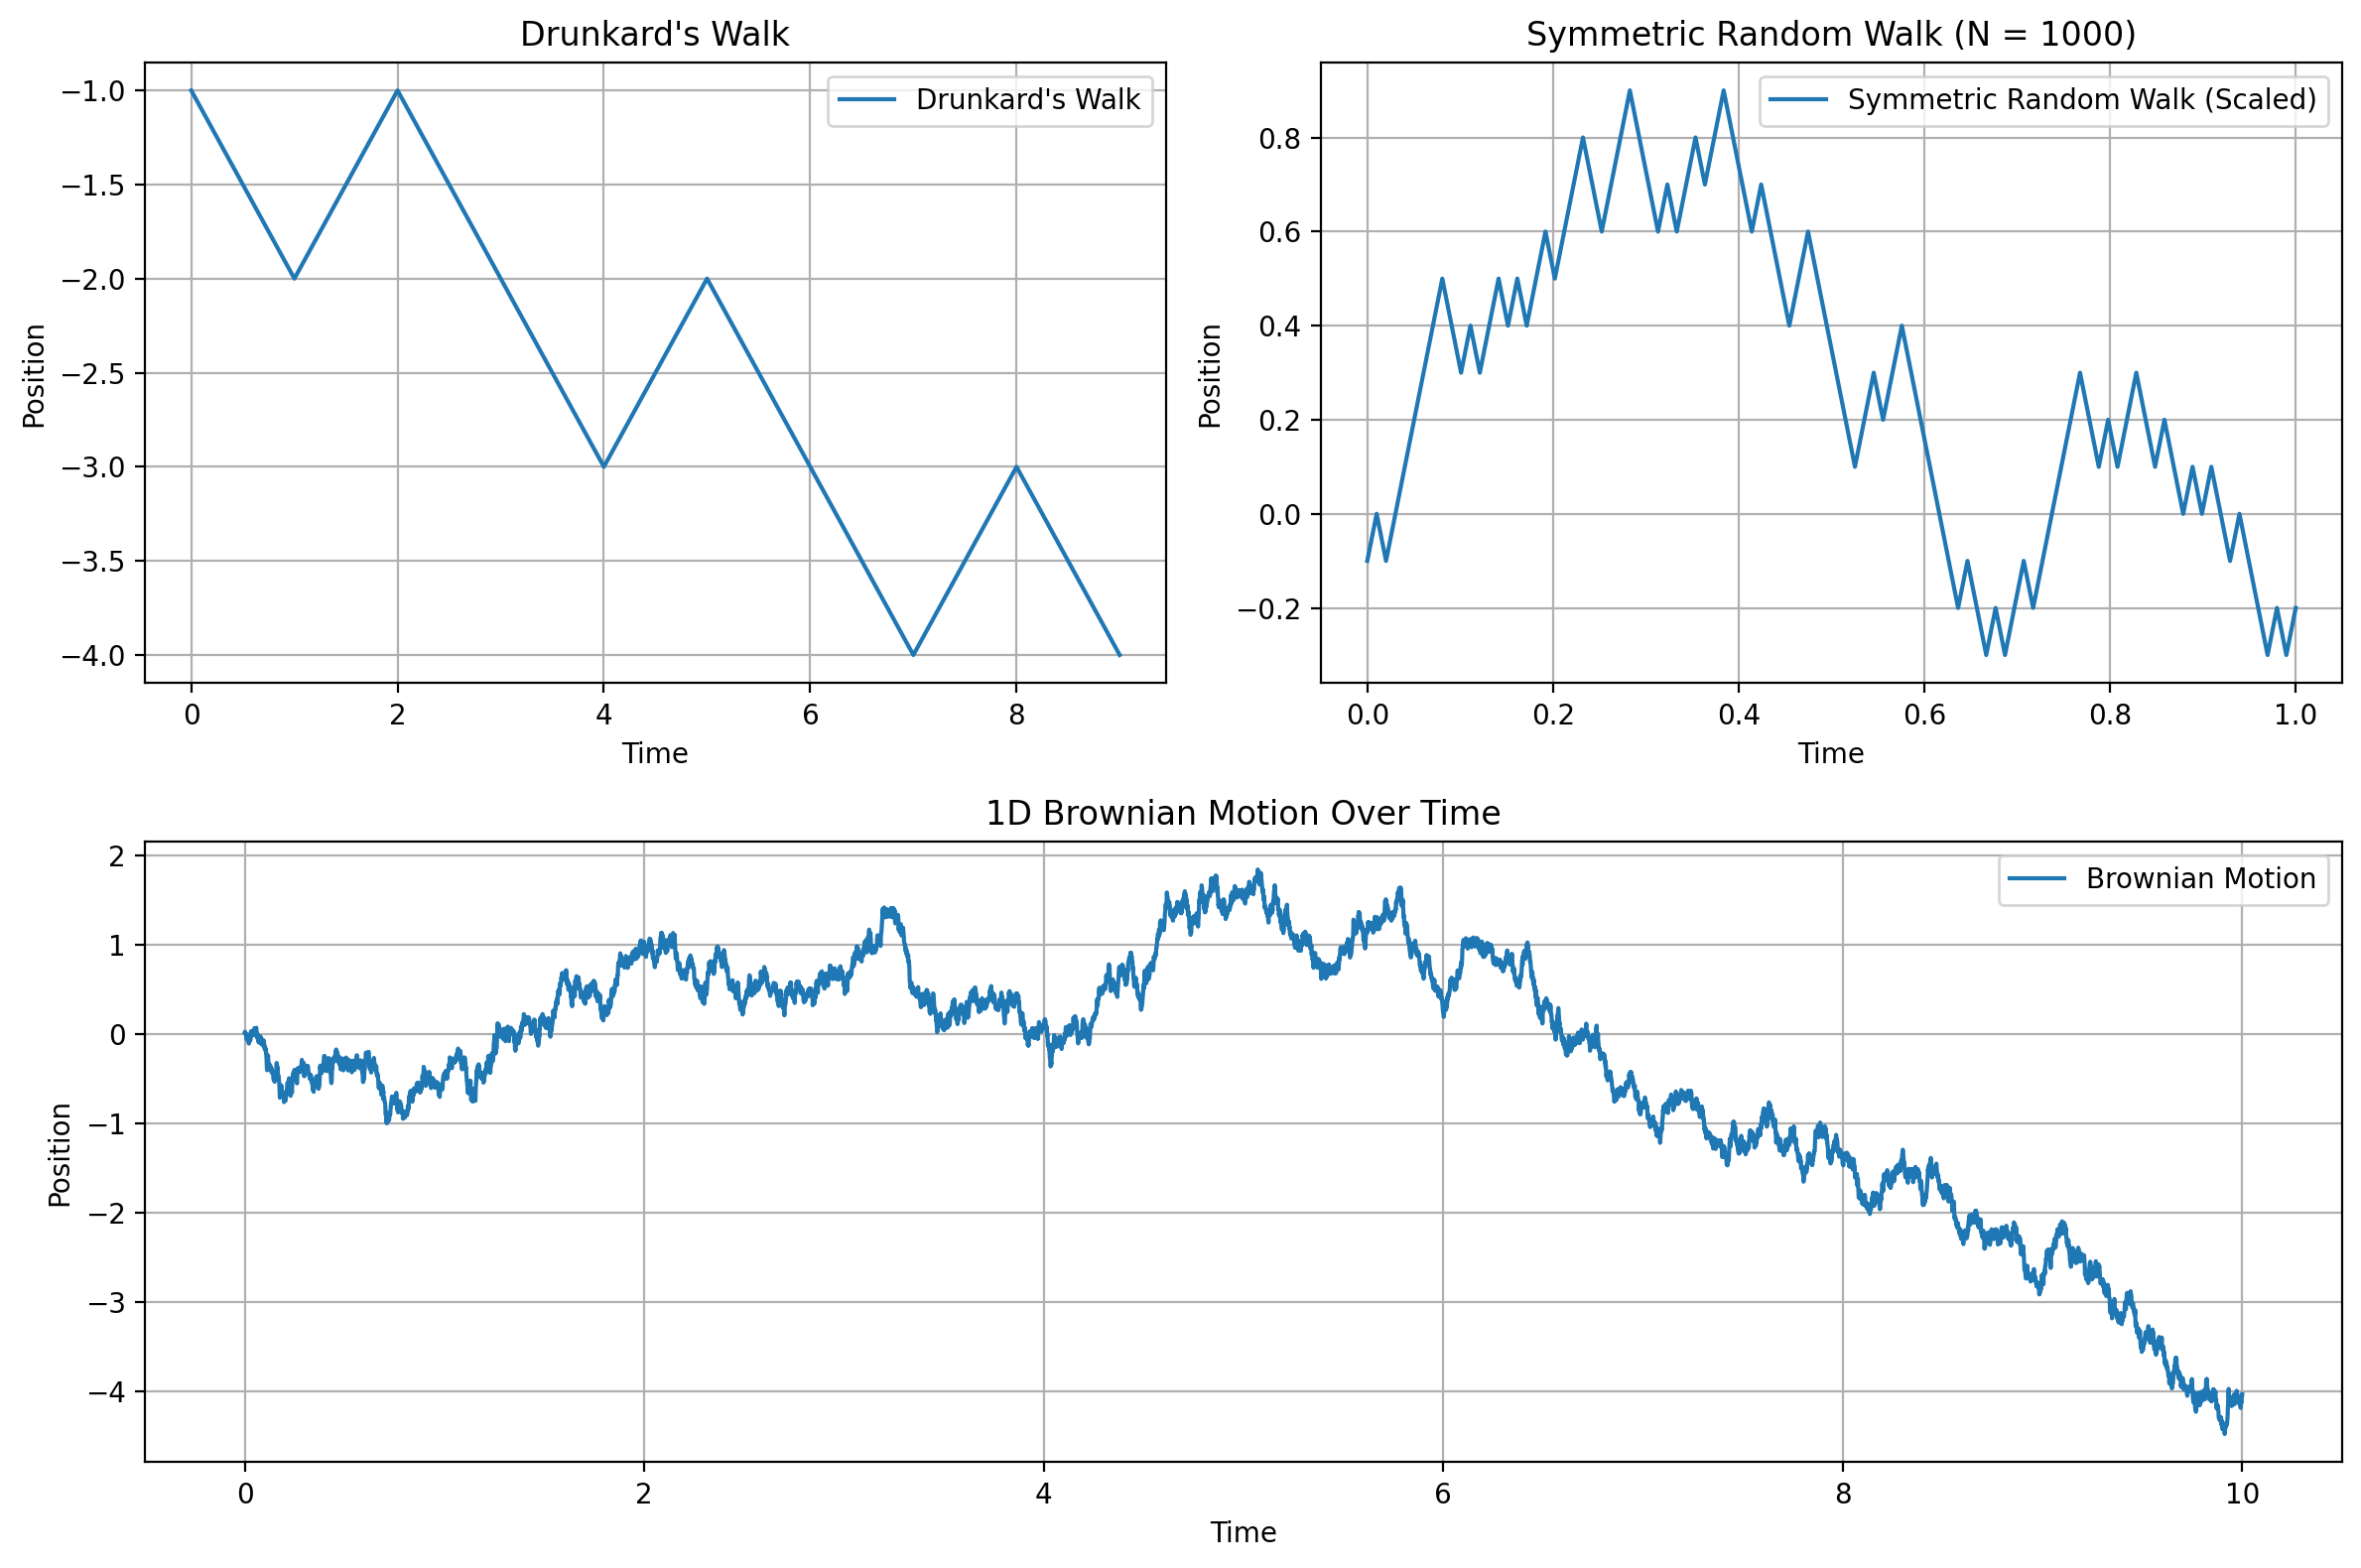
\includegraphics[width=0.5\linewidth]{Images/Drunkard's Walk.png}
    \caption{From My REU Paper}
\end{figure}
We wish to show that $\sum_{n=1}^\infty p^n(0,0) = \infty.$ Since the parity of $n$ must be even, it suffices to show that $\sum_{n=1}^\infty p^{2n}(0,0).$ After a bit of thought, and by using Stirling's Formula above,
\[p^{2n}(0,0) = \bbP\{X_{2n} = 0 \mid X_0 = 0\} = \frac{\binom{2n}{n}}{2^{2n}} \sim \frac{\sqrt{4\pi n}(\frac{2n}{e})^{2n}}{2\pi n (\frac{n}{e})^{2n}}2^{-2n} = \frac{1}{\sqrt{\pi n}}.\] Hence, the infinite series diverges and so the random walk on $\bbZ$ is recurrent. Indeed, it is null recurrent. 

For $d = 2,$ we want to do something similar. Fix $j.$ There must be $j$ steps to the right and $j$ steps to the left in order to get back to the origin. Thus, there must be $n-j$ steps up and $n-j$ steps down. Thus, there are 
\[\frac{2n!}{j!^2(n-j)!^2}\] of such combinations.
\[p^{2n}(0,0) = \frac{\sum_{j=0}^{n}\frac{(2n)!}{(j!)^2 (n-j)!^2}}{4^{2n}} = \frac{1}{4^{2n}}\frac{(2n)!}{n!^2}\sum_{j=0}^n \left(\frac{n!}{j! (n-j)!}\right)^2 = \frac{1}{4^{2n}}\binom{2n}{n}\sum_{j=0}^n \binom{n }{j}\binom{n}{n-j} = \frac{1}{4^{2n}} \binom{2n}{n}^2\] By Stirling's approximation,
\[p^{2n}(0,0)   = \frac{1}{4^{2n}} \binom{2n}{n}^2\approx \frac{1}{\pi n} \implies \sum_{n=0}^\infty p^{2n}(0,0) = \infty,\] and thus the random walk is null recurrent.


For $d\geq 3,$ it can be shown that $p^{2n} = \left(\frac{1}{\sqrt{\frac{2\pi n}{d}}}\right)^d$

\end{proof}


\newpage
\subsection{Monday, Apr 14: Branching Processes}
Let $\{X_n\}$ denote the size of the population at time $n.$ Independent of the rest, each individual produces some number of offspring according to an offspring distribution $\{p_k\}.$ We remark that 
$\{p_k\}_{k\geq 0}$ satisfies $p_k \geq 0$ for all $k$ and $\sum_{k=0}^\infty p_k = 1.$ Informally, $p_k$ represents the probability of an individual producing $k$ children. Then if each $n$ represents a new generation where each previous generation dies of, then 
\[X_{n+1} = \sum_{j=1}^{X_n} \xi_j,\] where the $\xi_j$ are conditionally independent given $X_n$ with 
\[\bbP\{\xi_j  =k \mid X_n = x\} = p_k.\] Thus, $\xi_j$ is how many offspring individual $j$ produces. We are interested in the extinction probability, which is formally denoted by 
\[a:= \bbP\{\exists n\geq 1 \text{ s.t. } X_n = 0 \mid X_0 = 1\}.\] Denote the mean of the offspring distribution of each individual by 
\[\mu:= \sum_{k=0}^\infty kp_k.\] Note that 
\[\bbE[X_{n+1} \mid X_n = m] = \sum_{j=1}^m \bbE[\xi_j] = \mu m.\] Then using the law of total expectation, \[\bbE[X_{n+1}] = \sum_{m=0}^\infty\bbE[X_{n+1} \mid X_n]\bbP\{X_n = m\} = \mu \sum_{m=0}^\infty m\bbP\{X_n = m\} = \mu \bbE[X_n],\] and so $\bbE[X_n] = \mu^n \bbE[X_0].$

\begin{prop}
    If $\mu < 1,$ then $a = 1.$ 
\end{prop}
\begin{proof}
    Since $\bbE[X_n] \leq \mu^n \to 0$ as $n\to \infty,$ then $\bbE[X_n] \to 0.$ Consider that by Markov's inequality
    \[\bbP\{X_n \neq 0\} = \bbP\{X_n \geq 1\} \leq \bbE[X_n]\to 0,\] and so $\bbP\{X_n = 0\} \to 1$ as $n\to \infty.$ 
\end{proof}

\begin{rem}
    If $X_1 = k,$ then by independence, $\bbP\{\text{extinction} \mid X_1 = k\} = a^k.$ Thus, 
    \[a = \bbP\{\text{extinction} \mid X_0 = 1\} = \sum_{k=0}^\infty \bbP\{X_1 = k\}\bbP\{\text{extinction} \mid X_1 = k\} = \sum_{k=0}^\infty p_k a^k.\]
\end{rem}

\begin{defn}
    Let $Y$ be a random variable taking values in $\{0,1,2,\dots\}.$ Then the \textbf{generating function} for $Y$ is given by 
    \[\phi : [0, \infty) \to [0,\infty), \quad \phi(s) = \phi_Y(s) = \bbE[s^y] := \sum_{k=0}^\infty \bbP\{Y = k\}s^k\]
\end{defn}
\begin{rem}
    (Basic Properties of $\phi$):
    \begin{enumerate}
        \item We allow $\phi(s) = \infty,$ but we have that $\phi(s) < \infty$ for $s\in [0,1]$ since it is bounded above by a converging geometric series. 
        \item $\phi (1) = 1$ and $\phi(0) = p_0.$ 
        \item The derivative has meaning:
        \[\phi'(s) = \sum_{k=1}^\infty \bbP\{Y = k\} k s^{k-1} \implies \phi'(1) = \bbE[Y].\]
        \item If $Y_1, \dots Y_m$ are independent random variables, then 
        \[\phi_{Y_1 + \dots + Y_m}(s) = \bbE[S^{Y_1 + \dots + Y_m}] = \prod_{j=1}^m \phi_{Y_j}(s)\]
    \end{enumerate}
    \end{rem}

\begin{prop}
    Let $\phi$ be the generating function for $p_k.$ Let $\phi^{(n)} = \phi \circ \phi \dots \circ \phi$ ($n$ times). Then
    \[\phi_{X_n}(s) = \phi^{(n)}(s)\]
\end{prop}
\begin{proof}
    It suffices to show that $\phi_{X_{n+1}}(s) = \phi_{X_{n}}(\phi(s)).$ By definition, 
    \begin{align*}
        \phi_{X_{n+1}}(s) &= \sum_{k=0}^\infty \bbP\{X_{n+1} = k\}s^k\\
        &= \sum_{k=0}^\infty \sum_{j=0}^\infty \bbP\{X_{n+1} = k \mid X_n = j\}\bbP\{X_n = j\} s^k\\
        &= \sum_{j=0}^\infty \bbP\{X_n = j\}\sum_{k=0}^\infty \bbP\{X_{n+1} = k \mid X_n = j\}s^k\\
        &= \sum_{j=0}^\infty \bbP\{X_n = j\} \phi(s)^j\\
        &= \sum_{j=0}^\infty \bbP\{X_n = j\} \phi(s)^j\\
        &= \phi_{X_n}(\phi(s))
    \end{align*}
\end{proof}

\newpage
\subsection{Wednesday, Apr 16: Extinction Probabilities}
Recall the generating function 
\[\phi_X (s) = \sum_{k=0}^\infty p_k s^k\]
\begin{prop}
    The extinction probability is the smallest positive solution for which $\phi(s) = s$ given that $0 < p_0 < 1.$
\end{prop}
\begin{proof}
    Since the set $\{s: \phi(s) = s\}$ is closed by continuity, then since $p_0 = \phi(0) = 0,$ then $0 \notin S.$ Thus, the set has a smallest positive element $s_0.$ Since $\phi(1) = 1,$ then $s_0 \leq 1.$ We claim that 
    \[\phi_{X_n}(0) < s_0,\quad  n\geq 0\] This is clear for $n=0$ since $\phi_{X_0}(0) = 0.$ If this is true for $n,$ that $\phi_{X_n}(0) < s_0,$ then by our proposition 14, and the fact that $\phi$ is strictly increasing (the derivative is strictly increasing) we have that 
    \[\phi_{X_{n+1}}(0) = \phi(\phi_{X_n}(0)) < \phi(s_0) = s_0.\] Note that since $\phi_{X_n}(0) = \bbP\{X_n = 0\},$ then 
    \[a = \lim_{n\to \infty}\phi_{X_n}(0) \leq s_0.\] Since $\phi(a) = a,$ then $a = s_0.$
\end{proof}
\begin{prop}
    If $\mu >1,$ then $a<1.$ If $\mu \leq 1$ and $p_0 \neq 0,$ then $a = 1.$ In particular, the population will die with probability $1$ if, and only if, $\mu \leq 1$ and $p_0 \neq 0.$
\end{prop}
\begin{proof}
    Suppose $\mu = 1$ and $p_0 \neq 0.$ Note that 
    \[\phi''(s) = \sum_{k=2}^\infty k(k-1)p_k s^{k-2}.\] If $p_0 \neq 0$ and $\mu = 1,$ then we claim that $p_k >0$ for some $k \geq 2.$ If not, then $\mu = p_1 < 1.$ Then $\phi''(s) >0.$ Recall that $\phi(1) = 1$ and $\phi'(1) = \mu.$ Thus, $\phi'(s) < \mu$ for all $s\in [0,1).$ If $\mu = 1,$ then 
    \[1 - \phi(s) = \int_s^1 \phi'(t)dt < \int_s^1 \mu dt  = 1-s.\] Thus, $\phi(s) >s$ for all $s\in [0,1).$ Thus, $a = 1. $ 

    If $\mu >1,$ then $\phi'(1) >1,$ $\phi(1) = 1.$ Then there exists $s<1$ such that $\phi(s) < s.$ Since $\phi(0) >0,$ the continuity of $t \mapsto \phi(t)-t$ implies by the IVT there is a $t\in (0,1)$ such that $\phi(t) = t.$ Hence, $a<1. $
\end{proof}

\begin{defn}
    We say that a branching process is \textbf{subcritical} if $\mu <1,$ \textbf{critical} if $\mu  = 1,$ and \textbf{supercritical} if $\mu >1.$ 
\end{defn}

\begin{exmp}
    Suppose $p_0 = \frac{1}{10},$ $p_1 = \frac{3}{5},$ and $p_2 = \frac{3}{10},$ then 
    \[\mu = \frac{1}{10} + \frac{3}{5} + \frac{6}{10} = \frac{12}{10} >1.\] Note that 
    \[\phi(s) = \sum_{k=0}^3 p_ks^k = \frac{1}{10} + \frac{3}{5}s + \frac{3}{10}s^2.\] We want the smallest positive solution to $\phi(s) = s.$ Solving gives $ a = \frac{1}{3}. $
\end{exmp}

\begin{exmp}
    Bacteria reproduce by cell division. In one unit of time, bacterium will either die (w.p. $\frac{1}{4}$,) stay the same (w.p. $\frac{1}{4}$), or split in 2 (w.p. $\frac{1}{2}$). At time $n = 0,$ the population starts with $100$ bacteria. 

    We can interpret this as the following: If a bacteria dies, then it produces three offspring?
    Then 
    \[\phi(s) = \sum_{k = 0}^\infty p_k s^k,\] where 
    \[p_1 = \frac{1}{4}, p_2  = \frac{1}{4}, p_3 = \frac{1}{2}\]
    \[\phi(s)= \frac{1}{4} + \frac{1}{4}s + \frac{1}{2} s^2, \quad Y_1, \dots, Y_{100}, \quad \phi_{Y_1 + \cdots Y_{100}} = (\tilde{\phi})^{100}.\] Then 
    \[\mu = \frac{1}{4} + 1 >1.\] Thus, we need to solve 
    \[\phi(s) - s = 0 \implies s = \frac{1}{2}\] for each one. Thus, by independence,
    \[ a = \frac{1}{2^{100}}\]
\end{exmp}
\newpage

\subsection{Friday, Apr 18: Poisson Processes}

\begin{defn}
    A random variable $Y$ is \textbf{Poisson} with parameter $\lambda$ if for all $k\geq 0,$ we have that 
    \[\bbP\{Y  = k\} = e^{-\lambda}\frac{\lambda^k}{k!}\]
\end{defn}
\begin{rem}
    Recall that $\bbE[Y] = \Var[Y] = \lambda.$ 
\end{rem}
\begin{prop}
    Suppose $Y_1,Y_2$ are independent Poisson random variables with parameters $\lambda_1, \lambda_2,$ respectively. Then $Y_1 + Y_2 \sim \text{Poisson}(\lambda_1 + \lambda_2).$
\end{prop}

We motivate the Poisson process with an example:
\begin{exmp}
    Suppose that in a phone line, calls occur at the same rate $\lambda$ at all hours in a day. The number of calls during disjoint time intervals are independent. Let $X_t$ be the number of calls at (or before) time $t.$  
\end{exmp}

\begin{defn}
    The \textbf{Poisson process} with rate $\lambda$ is the continuous time stochastic process $\{X_t\}_{t\geq 0}$ such that:
    \begin{itemize}
        \item $X_0 = 0;$
        \item For any times $0 \leq s_1 \leq t_1 \leq s_2 \leq \cdots \leq s_k \leq t_k,$ the random increments 
        \[X_{t_j} - X_{s_j} \sim \text{Poisson}(\lambda (t_j - s_j))\] are independent
    \end{itemize}
\end{defn}

\begin{defn}
    A random variable $T \in [0, \infty)$ has the exponential distribution with parameter $\lambda$ if 
    \[\bbP\{T \geq t\} = e^{-\lambda}\]
\end{defn}
Recall that $\bbE[T] = \frac{1}{\lambda}$ and $\Var[T] = \frac{1}{\lambda^2}.$

\begin{rem}
    We could alternatively describe a Poisson process in terms of arrival times. Let $\tau_0 = 0$ and let $\tau_j = \inf\{t \geq 0 \mid X_t = j\}$ be the time of the $j$th call. Then $X_t = \max\{j \mid \tau_j \leq t\}$ is the number of calls before time $t.$ 
\end{rem}

\begin{prop}
    The arrival times $\tau_j - \tau_{j-1}$ for $j = 1,2,3,\dots$ are i.i.d. and each has exponential distribution with parameter $\lambda.$
\end{prop}
\begin{proof}
    Note that $\tau_0 = 0,$ and 
    \begin{align*}
        \bbP\{\tau_1 > t\} = \bbP\{X_t = 0\} = \frac{e^{-\lambda }\lambda^k}{k!} = e^{-\lambda}.
    \end{align*}
    Then $\tau_1 \sim \text{Exp}(\lambda).$ Note that $\tau_1$ is a stopping time for $\{X_t\}$ and $\{T_{s + t} - X_t\}_{s\geq0}$ is a Poisson process independent of $\{X_s\}_{s\leq t}.$ By the strong Markov property, 
    \[\{X_{s + \tau_1} - X_{\tau_1}\}_{s\geq 0}\] is Poisson and independent of $\{X_{s}\}_{s\leq \tau_1}.$ In particular, $\tau_2 - \tau_1$ is independent of $\tau_1$ and has the same distribution.
\end{proof}

\begin{exmp}
    Suppose $\{X_t\}_{t\geq 0}$ is a Poisson process with rate $\lambda.$ Then 
    \[\bbE[X_2 \mid X_1] = X_1 + \lambda\]
\end{exmp}

\newpage
\subsection*{Monday, Apr 21: Continuous Time Markov Process}
\begin{prop}
    (Minimum Property) Suppose $T_1, \dots, T_n$ are independent exponential r.v. with parameters $\lambda_1, \dots, \lambda_n$ (respectively). Then $\min\{T_1, \dots, T_n\}$ is an exponential random variable with parameter $\lambda_1 + \cdots + \lambda_n.$ Moreover, for any $j  = 1,2,3\dots, n,$ we have that
    \[\bbP\{T_j = \min\{T_1, \dots, T_n\}\} = \frac{\lambda_j}{\lambda_1 + \dots + \lambda_n}\]
\end{prop} 
\begin{proof}
    We have that 
    \begin{align*}
        \bbP\{T_{(1)}\geq t\} &= \bbP\{T_1, \geq t, T_2 \geq t, \dots , T_n \geq t\}\\
        &= \bbP\{T_1 \geq t\}\cdots \bbP\{T_n \geq t\}\\
        &= e^{-\lambda_1 t}\cdots e^{-\lambda_n t}\\
        &= e^{-(\lambda_1 + \cdots + \lambda_n)t}.
    \end{align*}
    For the second claim, we have that if $j=1,$ then 
    \begin{align*}
        \bbP\{T_1 = T_{(1)}\} &= \bbP\{T_j \geq T_1, \;\forall j = 1,2,\dots, n\}\\
        &= \bbE[\bbP\{T_j \geq T_1, \;\forall j = 1,2,\dots, n \mid T_1\}]\\
        &=  \bbE[e^{-(\lambda_1 + \dots, \lambda_n)T_1}]\\
        &= \lambda_1\int_{0}^\infty e^{-(\lambda_1 + \dots, \lambda_n)t}dt\\
        &= \frac{\lambda_1}{\sum_{j=1}^n\lambda_j}
    \end{align*}
    
\end{proof}

Suppose $S$ is a finite state space. We wish to define a stochastic process $\{X_t\}_{t\geq 0}$ taking values in $x.$ For distinct $x,y \in S,$ there exists some rates $\alpha(x,y) \geq 0 $ that specify how frequently we jump from $x$ to $y$.
\begin{rem}
    For $y \in S$ with $\alpha(x,y) \neq 0,$ let $T_1$ be an exponential r.v. with parameter $\alpha(x,y).$  Let $T = \min_y T_y.$ By the minimum property, $T\sim \exp(\alpha(x)),$ where $\alpha(x) = \sum_{y \in S\sm \{x\}}\alpha(x,y).$ Moreover, we have that 
    \[\bbP\{X_T = y\} = \frac{\alpha(x,y)}{\alpha(x)}\]
\end{rem}

\begin{prop}
(The Markov Property)
    Let $t \geq 0$ and $x\in S.$ The conditional distribution of $\{X_{t + s}\}_{s\geq 0 }$ given $\{X_t = x\}$ (and everything before time $t$), is the same as the distribution of $\{X_s\}$ started from $x.$ 
\end{prop}

Now, we aim to write down a transition matrix for this process. 
\begin{defn}
    Define the \textbf{$t-$time transition probabilities} to be 
    \[p_t(x,y) = \bbP\{X_t = y  \mid X_0 = x\}\] and label $S = \{1,2,\dots, N\}$ and define the \textbf{$t-$time transition matrix} as 
    \[P_t = \begin{pmatrix}
        p_t(x,y)
    \end{pmatrix}_{x,y = 1,2,\dots, N}\]
\end{defn}
\begin{rem}
For $x\neq y,$ we know that by the Markov Property, 
\[\bbP\{X_{t  + \epsilon} = y \mid X_t = x\} = \bbP\{X_\epsilon = y \mid X_0 = x\} \approx \bbP\{T_y < \epsilon\} = 1 - e^{\alpha(x,y)\epsilon}  = \alpha(x,y)\epsilon + O(\epsilon^2).\] Thus, 
\[\bbP\{X_{t + \epsilon} \neq x \mid X_t = x\} = \sum_{y \sm \{x\}}\alpha(x,y)\epsilon  + O(\epsilon^2) = \alpha(x)\epsilon + O(\epsilon^2).\]

Informally, \[\frac{d}{dt}p_t(x,y) = \lim_{\epsilon \to 0} \frac{1}{\epsilon}\left(\bbP\{X_{t + \epsilon }  = y \mid X_0 = x\} - \bbP\{X_t = y \mid X_0 = x\}\right) = \cdots = \sum_{z\in S\sm \{y\}}\alpha(x,y)p_t(x,z) - \alpha(y)p_t(x,y)\]

In matrix form, 
\[\frac{d}{dt}P_t = P_tA,\] where $A$ is the $N\times N$ whose $x,y$ entry is $\alpha(x,y)$ if $x\neq y$ and $-\alpha(x)$ if $x = y.$ Note that $p_0 (x,x) = 1$ and $p_0(x,y) =0.$ Thus, $P_0 = I.$ The solution to this ODE gives 
\[P_t = e^{tA}\]

\end{rem}

\newpage
\subsection{Wednesday, Apr 23: Midterm}

\newpage
\subsection{Friday, Apr 25: $t-$Time Transition Matrix}
\begin{rem}
    Since $P_t = e^{tA},$ we have that 
    \[e^{tA} = \sum_{n=0}^\infty \frac{(tA)^n}{n!}.\] Thus, if $A = QDQ^{-1}$ and so 
    \[e^{tA} = Q e^{tD}Q^{-1}.\] Note that if $D$ is diagonal with entries $\lambda_1, \dots, \lambda_m,$ then $e^{tD}$ is the diagonal matrix with diagonal entries $e^{t\lambda_1}, \dots, e^{t\lambda_m}.$

    The matrix $A$ is called the \textbf{infinitesimal generator} for the Markov Chain.
\end{rem}

\begin{exmp}
    Consider the Markov Chain with state space $S = \{0,1\}$ and rates 
    \[\alpha(0,1) = 2, \quad \alpha(1,0) = 3.\]
    Then 
    \[A = \begin{pmatrix}
        -2 & 2\\
        3 & -3
    \end{pmatrix}\] Then 
    \[A - \lambda I =  \begin{pmatrix}
        -2 - \lambda & 2  \\
        3   & -3 - \lambda
    \end{pmatrix}\] Then 
    \[|A - \lambda I | = (-2 - \lambda)(-3 - \lambda) - 6 \implies \lambda_1 = -5, \lambda_2 = 0.\] Then finding the null space $E_{-5}$ is 
    \[E_{-5} = \{v \mid (A - \lambda_{-5})v = 0\}\] which is formed by $v_5= (-2,3).$ Similarly, $v_0 = (1,1).$ Thus, 
    \[D = \begin{pmatrix}
        -5 & 0\\
        0 & 0
    \end{pmatrix}\quad Q = \begin{pmatrix}
        -2 & 1 \\
        -3 & 1
    \end{pmatrix} \quad Q^{-1} = \] and so 
    \[P_t = QDQ^{-1}= \begin{pmatrix}
        -2 & 1 \\
        -3 & 1
    \end{pmatrix} \begin{pmatrix}
        e^{-5t} & 0\\
        0 & 1
    \end{pmatrix}\begin{pmatrix}
        -2 & 1 \\
        -3 & 1
    \end{pmatrix}^{-1} = \frac{1}{5}\begin{pmatrix}
        3 + 2e^{-5t} & 2- 2e^{-5t}\\
        3 - 3e^{-5t} & 2 + 3e^{-5t}
    \end{pmatrix}\]
    Then 
    \[\bbP\{X_1 = 1 \mid X_0 = 0\} = \frac{2 - 2e^{-5t}}{5}\]
\end{exmp}

\begin{defn}
    A continuous time Markov Chain is \textbf{irreducible} if $p_t(x,y) >0$ for all $x,y \in S.$ and for all $t>0.$
\end{defn}
\begin{defn}
    A function $\pi: S \to [0,1]$ with $\sum_{x \in S}\pi_x = 1$ is an \textbf{invariant/stationary distribution} for $\{X_t\}$ if the following is true:
    \begin{itemize}
        \item If $X_0$ has distribution $\pi,$ then $X_t$ has distribution $\pi$ for all $t\geq 0.$
        \item It satisfies \[\frac{d}{dt}\pi P_t = 0 \iff \frac{d}{dt}\pi e^{tA} = 0 \iff \pi A = 0.\]
    \end{itemize}
\end{defn}

\begin{prop}
    If $\{X_t\}$ is irreducible, then there exists a unique stationary distribution $\pi$ for $\{X_t\}$ which satisfies, for any $x,y \in S,$
    \[\lim_{t\to \infty} p_t(x,y) = \pi_y\]
\end{prop}
\begin{exmp}
    It is easy to see that in the example above, 
    \[\pi = \begin{pmatrix}
        \frac{3}{5} & \frac{2}{5}
    \end{pmatrix}\]
\end{exmp}

\newpage
\subsection{Monday, Apr 28: Conditional Expectation}

\begin{rem}
    Suppose $X$ and $Y$ are r.v. taking values in countable sets $S,T \subset \bbR.$ For $x \in S$ and $y \in T,$ let 
    \[f(x,y) = \bbP\{X = x, Y = y\}.\] Then the \textit{conditional expectation} is 
    \[\bbE[X \mid Y = y] = \sum_{x \in S}x \bbP\{X = x \mid Y = y\} = \frac{\displaystyle\sum_{x\in S}s f(x,y)}{\displaystyle\sum_{x\in S}f(x,y)}.\] Moreover, we define the random variable
    \[\bbE[X \mid Y] = \frac{\displaystyle\sum_{x \in S} xf(x,y)}{\displaystyle\sum_{x\in S}f(x,y)}\]
\end{rem}

\begin{defn}
    Let $X,Y$ be random variables with $X$ taking values in $\bbR$ and with $\bbE[ | X|] < \infty.$ The \textbf{conditional expectation} $\bbE[X \mid Y]$ is the unique random variable  that satisfies the following:
    \begin{enumerate}
        \item $\bbE[X \mid Y]$ is a function of $Y.$
        \item If $F(y)$ is a function of $y$ taking values in $\bbR$ and $\bbE[ |F(y) | ] < \infty,$ then 
        \[\bbE[X \mid F(Y)] = \bbE[\bbE[X \mid Y] \mid F(y)]\]
    \end{enumerate}
\end{defn}

Suppose $\bbE[|X|] < \infty$ for any random variable talked about in this class.
\begin{defn}
 Let $\{X_t\}_{t∈T}$ be a stochastic process. We say that the \textbf{natural filtration} of $X_t$ is the sigma algebra generated by $Y_t$. That is,
 $\mathcal{F}_t =\sigma(Y_1,Y_2,...,Y_t)$.
\end{defn}
We note that the natural filtration of $X_0, \dots, X_n$ is the information contained in these random variables. 
\begin{rem}
    Moreover, 
    \[\bbE[X \mid \mathcal{F}_n] = \bbE[Y_0, \dots, Y_n]\]
 and we say that $X$ is $\mathcal{F}_n-$measurable if it is a function of $Y_0, \dots, Y_n$
 \end{rem}
 \begin{prop}
     $\bbE[X \mid \mathcal{F}_n]$ is the unique real valued random variable satisfying the following:
     \begin{enumerate}
         \item $\bbE[X \mid \mathcal{F}_n]$ is $\mathcal{F}_n$ measurable.
         \item $\bbE[X \mid Z] = \bbE[\bbE[X \mid \mathcal{F}_n] \mid Z]$
     \end{enumerate}
 \end{prop}

\begin{prop}(Linearity) Suppose $X_1, X_2$ are real valued r.v.s and $a,b \in \bbR.$ Then 
\[\bbE[aX_1 + bX_2 \mid \mathcal{F}_n] =  a\bbE[X _1 \mid \mathcal{F}_n] +  b\bbE[ X_2 | \mathcal{F}_n]\]
\end{prop}
\begin{proof}
    If $Z$ is $\mathcal{F}_n-$measurable, then  $\bbE[aX_1 + bX_2 \mid Z] = \bbE[\bbE[aX_1 + bX_2 \mid \mathcal{F}_n] \mid Z].$ Let
    \[W:= a\bbE[X_1 \mid \mathcal{F}_n] + b\bbE[X_2 \mid \mathcal{F}_n]\] Then 
    \begin{align*}
        \bbE[W \mid Z] &= \bbE[a \bbE[X_1 \mid \mathcal{F}_n] + b\bbE[X_2 \mid \mathcal{F}_n] \mid Z]\\
        &= \bbE[a \bbE[X_1 \mid \mathcal{F}_n]\mid Z] + \bbE[b\bbE[X_2 \mid \mathcal{F}_n]\mid Z]\\
        &= a\bbE[X_1 \mid Z] + b\bbE[X_2 \mid Z]\\
        &= \bbE[aX_1 + bX_2 \mid Z].
    \end{align*}
    Because conditional expectation is unique, we are done.
\end{proof}
\begin{prop}
    Suppose $X$ is $\mathcal{F}_n-$measurable, then $\bbE[X \mid \mathcal{F}_n] = X.$
\end{prop}
\begin{prop}
    If $X$ is independent from $\mathcal{F}_n,$ then 
    \[\bbE[X \mid \mathcal{F}_n] = \bbE[X]\]
\end{prop}
\begin{prop}
    If $Z$ is $\mathcal{F}_n-$measurable, then 
    $\bbE[ZX \mid \mathcal{F}_n] = Z\bbE[X \mid \mathcal{F}_n].$
\end{prop}
\begin{exmp}
    Let $X_1, X_2,\dots$ be i.i.d r.vs with mean $\mu.$ Then if $m\geq n,$ 
    \[\bbE[X_1  + \dots  + X_n \mid \mathcal{F}_m] = X_1 + \dots + 
 X_n.\] If $m < n,$ then 
 \begin{align*}
  \bbE[X_1 + \dots + X_n \mid \mathcal{F}_m] &= \bbE[X_1 + \dots 
 + X_m \mid \mathcal{F}_m] + \bbE[X_{m+1} + \dots + X_n \mid \mathcal{F}_m]   \\
 &= X_1 + \dots + X_m + \bbE[X_{m+1} \mid \mathcal{F}_m] + \dots  + \bbE[X_n \mid \mathcal{F}_m]\\
 &= X_1 + \dots + X_m + \bbE[X_{m+1}] + \dots  + \bbE[X_n ]\\
 &= X_1 + \dots + X_m + (n-m)\mu
 \end{align*}
 
\end{exmp}

\begin{exmp}
    Let $X_1, \dots, X_n$ be i.i.d. with mean $0$ and variance $\sigma^2.$ Then 
    \begin{align*}
        \bbE[(X_1 + \dots + X_n)^2 \mid \mathcal{F}_m] &= S_m^2 + (n-m)\sigma^2.
    \end{align*}
\end{exmp}


\newpage
\subsection{Wednesday, Apr 30: Martingales}
\begin{defn}
    Let $\{X_t\}$ be a stochastic process. The \textbf{natural filtration} of $X_t$ is defined to be 
    \[\mathcal{F}_n = (X_1, \dots, X_n)\]
\end{defn}

\begin{defn}
    A stochastic process $\{M_n\}$ is called a martingale w.r.t. $\{\mathcal{F}_n\}$ if:
    \begin{enumerate}
        \item Each $M_n$ is $\mathcal{F}_n$ measurable.
        \item $\bbE[|M_n|] < \infty$ for all $n.$
        \item For each $m < n,$
        \[\bbE[M_n \mid \mathcal{F}_m] = M_m.\]
    \end{enumerate}
\end{defn}
\begin{rem}
    In particular, we can rewrite the Martingale Property to be $\bbE[M_n - M_m \mid \mathcal{F}_m] = 0.$ By the tower property, 

    \[\bbE[M_n] = \bbE[\bbE[M_n \mid \mathcal{F}_0]] = \bbE[M_0].\]
\end{rem}

\begin{prop}
    To prove $\bbE[M_n \mid F_m] = M_m$, it suffices to show that $\bbE[M_n \mid \mathcal{F}_{n-1}] = M_{n-1}$
\end{prop}
\begin{proof}
\[\bbE[M_n \mid \mathcal{F}_{n-2}] = \bbE[\bbE[M_n \mid \mathcal{F}_{n-1}]\mid \mathcal{F}_{n-2}] = \bbE[M_{n-1}\mid \mathcal{F}_{n-2}]= M_{n-2}\]
\end{proof}

\begin{exmp}
    Let $X_1, X_2, \dots$ be i.id. with mean $\mu,$ and let $\mathcal{F}_n$ be the natural filtration of $X_n.$ Let $S_0 = 0$ and $S_n = X_1 + \dots + X_n.$ Let $M_n = S_n - n\mu.$ 

    \begin{enumerate}
        \item The first property is inmediate.
        \item For any $n,$
        \[\bbE[|M_n|] \leq \bbE[|S_n|] + \mu n < \infty.\]
        \item For any $n,$
    \begin{align*}
        \bbE[M_n \mid \mathcal{F}_{n-1}] &= \bbE[(X_1 + \dots + X_n) - n\mu \mid \mathcal{F}_{n-1}]\\&= \bbE[M_{n-1} + (X_n - \mu) \mid \mathcal{F}_{n-1}]\\& = \bbE[M_{n-1} \mid \mathcal{F}_{n-1}] + \bbE[X_n - \mu \mid \mathcal{F}_{n-1}]\\& = M_{n-1}
    \end{align*}
    \end{enumerate}
\end{exmp}

\begin{exmp}
    Let $X_1, X_2, \dots$ be i.i.d. with mean $0$ and variance $\sigma^2.$ Let $\mathcal{F}_n$ be the natural filtration of $X_n.$ Let $M_n:= S_n^2 - n\sigma^2.$
    \begin{enumerate}
        \item Again, the first property is clear.
        \item For any $n,$
\[\bbE[|M_n|] \leq \bbE[S_n^2] + n\sigma^2 = \Var[S_n] - \bbE[S_n]^2 + n\sigma^2 = n\sigma^2 + n\sigma^2 < \infty\]
\item For any $n,$ we have (from Example 1.27)
\begin{align*}
    \bbE[M_n \mid \mathcal{F}_{n-1}] &= \bbE[S_n^2 - n\sigma^2 \mid \mathcal{F}_{n-1}]\\
    &= \bbE[S_n^2\mid \mathcal{F}_{n-1}] - n\sigma^2\\
    &= S_{n-1}^2 + \sigma^2 - \sigma^2 n\\
    &= M_{n-1}
\end{align*}
    \end{enumerate}
\end{exmp}

\begin{exmp}
    Let $Y_0, Y_1, \dots$ be a sequence of random variables and let $\mathcal{F}_n$ be the natural filtration. Let $X$ be a random variable such that $\bbE[|X|] < \infty,$ and let 
    \[M_n = \bbE[X \mid \mathcal{F}_n]\]
    \begin{enumerate}
        \item Clealry, $M_n$ is $\mathcal{F}_n$ measurable.
        \item For any $n,$
    \[\bbE[|M_n|] \leq \bbE[\bbE[|X| \mid \mathcal{F}_n]] = \bbE[|X|] < \infty.\]
    \item By the tower property,
\begin{align*}
    \bbE[M_n \mid \mathcal{F}_{n-1}] &= \bbE[\bbE[X \mid \mathcal{F}_{n}] \mid \mathcal{F}_{n-1}]\\
    &= \bbE[X \mid \mathcal{F}_{n-1}]\\
    &= M_{n-1}
\end{align*}
    \end{enumerate}
\end{exmp}


We know $\bbE[M_n] = \bbE[M_0]$ for any $n.$ Is this still true for a random time $\tau.$ 

\begin{rem}
    Let $\tau$ be a stopping time for $\{\mathcal{F}_n\}.$ Doob's Optional Stopping Theorem states that, under certain conditions, 
    \[\bbE[M_\tau] = \bbE[M_0]\]
\end{rem}
\begin{exmp}
(Gambler's ruin)
    Let $X_1, X_2, \dots$ be i.i.d with $\bbP\{X_i = 1\} = \bbP\{X_i = -1\} = \frac{1}{2}.$ Then $S_n = X_1 + \dots X_n$ is  a martingale by Example 1.28. Let $\tau := \min\{n \geq 0 \mid S_n = a \text{ or } S_n = -b\}.$
    DOST tells us that 
    \[\bbE[S_\tau] = \bbE[S_0] = 0,\] and thus 
    \begin{align*}
        0 &= \bbE[S_\tau]\\ &= a\bbP\{S_n = a\}  + (-b)\bbP\{S_n = -b\}\\
        &= a p_W - b p_L\\
        &= ap_W - b(1-p_W)
    \end{align*}
    and thus 
    \[p_W = \frac{b}{a + b}\]
\end{exmp}








\newpage
\section{Problem Sessions}
\subsection{Monday, Mar 31: Problem Session 1}
When do we run into the issue that $\lim_{n\to \infty}\pi P^n$ does not exist? 
\begin{enumerate}
    \item[(1)] If Period $> 1$
    \item[(2)] If there are multiple recurrence classes that are transient.
\end{enumerate}

Problems:
\begin{enumerate}
    \item Let $X_0, X_1, \dots$ be a Markov chain with state space $S = \{0, 1, 2, 3\}$, and with transition matrix
    \[
    \begin{bmatrix}
        \frac{1}{4} & 0 & \frac{1}{2} & \frac{1}{4} \\
        0 &  \frac{1}{5} & 0 & \frac{1}{5} \\
        0 & 1 & 0 & 0 \\
        \frac{1}{3} & \frac{1}{3} & 0 & \frac{1}{3}
    \end{bmatrix}.
    \]
    A new process is defined by $Z_n = 0$ if $X_n = 0$ or $1$ and $Z_n = X_n$ if $X_n = 2$ or $3$. Find $P(Z_{n+1} = 2 | Z_n = 0, Z_{n-1} = 2)$ and $P(Z_{n+1} = 2 | Z_n = 0, Z_{n-1} = 3)$. Is $Z_n$ a Markov chain?
    \begin{solution}
    \begin{align*}
        \bbP\{Z_{n + 1}= 2 \mid Z_n = 0, Z_{n-1} = 2\} &= \frac{\bbP\{Z_{n + 1} = 2, Z_{n} = 0, Z_{n-1} = 2\}}{\bbP\{Z_n = 0, Z_{n-1 } = 2\}}\\
        &= \frac{\bbP\{Z_{n + 1} = 2, Z_{n} = 0 \mid Z_{n-1} =2\}}{\bbP\{Z_n = 0 \mid Z_{n-1} = 2\}}\\
        &= 0
    \end{align*}
    \begin{align*}
        \bbP\{Z_{n + 1} = 2 \mid Z_n = 0, Z_{n-1} = 3\} &= \frac{\bbP\{Z_{n + 1} = 2, Z_{n} = 0 \mid Z_{n-1} =3\}}{\bbP\{Z_n = 0 \mid Z_{n-1} = 3\}}\\
        &= \frac{\bbP\{X_n = 2, X_n = 0 \mid X_{n-1} = 3\} +\bbP\{X_n = 2, X_n = 1 \mid X_{n-1} = 3\}}{\bbP\{X_n = 0 \mid X_{n-1} =3\} + \bbP\{X_{n} = 1 \mid X_{n-1} = 3\}}\\
        &= \frac{\frac{1}{3}\frac{1}{2} + 0}{\frac{1}{6} + \frac{1}{6}}\\
        &= \frac{1}{4}
    \end{align*}
    Thus, $\{Z_n\}$ is not a Markov chain
    \end{solution}

    \item We repeatedly roll two four-sided dice with numbers 1, 2, 3, and 4 on them. Let $Y_k$ be the sum on the $k$-th roll, $S_n = Y_1 + Y_2 + \dots + Y_n$ be the total of the first $n$ rolls, and $X_n = S_n (\text{ mod } 6)$. Find the transition matrix for $\{X_n\}$.
    \begin{solution}
        $\{X_n\}$ is a Markov process because it only depends on the current state $S_n,$ as you can figure out the next turn only from this, since 
        \[X_{n + 1} = S_{n + 1}\text{ mod } 6 = (S_{n} + Y_{n + 1})\text{ mod } 6= S_n \text{ mod } 6 + Y_{n + 1}\text{ mod } 6 = X_n + Y_{n+1}\text{ mod } 6\] 
        \[P = \begin{bmatrix}
            \frac{3}{16} & \frac{1}{8} & \frac{1}{8} & \frac{1}{8} & \frac{3}{16} & \frac{1}{4}\\
             \frac{1}{4} & \frac{3}{16}& \frac{1}{8} & \frac{1}{8} & \frac{1}{8} & \frac{3}{16} \\
             \frac{3}{16} & \frac{1}{4} & \frac{3}{16}& \frac{1}{8} & \frac{1}{8} & \frac{1}{8} \\
             \frac{1}{8} & \frac{3}{16} & \frac{1}{4} & \frac{3}{16}& \frac{1}{8} & \frac{1}{8} \\
             \frac{1}{8} &\frac{1}{8} & \frac{3}{16} & \frac{1}{4} & \frac{3}{16}& \frac{1}{8} \\
             \frac{1}{8} &\frac{1}{8} &\frac{1}{8} & \frac{3}{16} & \frac{1}{4} & \frac{3}{16} 
        \end{bmatrix}\]
    \end{solution}

    \item Consider a Markov chain with states $S = \{0, \dots, N\}$ and transition probabilities $p(i, i+1) = p$, $p(i, i-1) = q$, for $1 \leq i \leq N-1$, where $p+q = 1$, $0 < p < 1$. Assume $p(0,1) = p(N, N-1) = 1$.
    \begin{enumerate}
        \item Draw a transition diagram for this chain.
        \begin{solution}
        In the following diagram, if you the probability  is above, then it is going to the right:
            \begin{center}
\begin{tikzpicture}[scale=1.2, every node/.style={draw, circle, inner sep=1pt}]
    \node (A) at (-4,0) {0};
    \node (B) at (-2,0) {1};
    \node (C) at (0,0) {$\cdots$}
    \node (D) at (2,0) {$N-1$};
    \node (E) at (4, 0) {$N$};

    \draw[->] (A) -- (B) node[midway, above] {\textcolor{red}{$1$}};
    \draw[->] (B) -- (A) node[midway, below] {\textcolor{red}{$q$}};
    \draw[->] (B) -- (C) node[midway, above] {\textcolor{red}{$p$}};
    \draw[->] (C) -- (B) node[midway, below] {\textcolor{red}{$q$}};
    \draw[->] (C) -- (D) node[midway, above] {\textcolor{red}{$p$}};
    \draw[->] (D) -- (C) node[midway, below] {\textcolor{red}{$q$}};
    \draw[->] (D) -- (E) node[midway, above] {\textcolor{red}{$p$}};
    \draw[->] (E) -- (D) node[midway, below] {\textcolor{red}{$1$}};
\end{tikzpicture}
\end{center}            
        \end{solution}
        \item Is the Markov chain irreducible? 
        \begin{solution}
Let $i,j \in [N],$ then we claim that $i \leftrightarrow j.$ Without loss of generality, suppose that $i < j.$ Suppose $j-i = N.$ Then $p(i,j)\geq p^N >0$ and $p(j,i) \geq q^N >0.$
        \end{solution}
        \item What is the period of this chain? 
        \begin{solution}
            The period has to be $2.$
        \end{solution}
    \end{enumerate}

    \item A taxicab driver moves between the airport $A$ and two hotels $B$ and $C$ according to the following rules. If he is at the airport, he will be at one of the two hotels next with equal probability. If at a hotel, then he returns to the airport with probability $\frac{3}{4}$ and goes to the other hotel with probability $\frac{1}{4}$.
    \begin{enumerate}
        \item Find the transition matrix for the chain.
        \begin{solution}
        \[
            P = \begin{bmatrix}
                0 & \frac{1}{2} & \frac{1}{2}\\
                \frac{3}{4} & 0 & \frac{1}{4}\\
                \frac{3}{4} & \frac{1}{4} & 0
            \end{bmatrix}\]
        \end{solution}
        \item Suppose the driver begins at the airport at time 0. Find the probability for each of his three possible locations at time 2 and the probability he is at hotel $B$ at time 3.
        \begin{solution}
        Squaring the matrix gives
                \[P^2 = \begin{bmatrix}
                    \frac{3}{4} & \frac{1}{8} & \frac{1}{8}\\
                    \frac{3}{16} & \frac{7}{16} & \frac{6}{16}\\
                    \frac{3}{16} & \frac{6}{16} & \frac{7}{16}
                \end{bmatrix}\]
                and so 
                \[p^2(A,A) = \frac{3}{4}, \quad p^2(B,A) = \frac{3}{16}, \quad p^2(C,A) = \frac{3}{16}\]
            Similarly, 
            \[p^3(B,A) = \frac{13}{32}\]
        \end{solution}
    \end{enumerate}

    \item At time $n = 0$, two ladybirds are placed at vertices $i$ and $j$ of a regular hexagon, whose vertices are labeled $1, \dots, 6$. At time $n = 1$, each of them moves, independently of the other, to one of the two adjacent vertices with probability $\frac{1}{2}$, and so on at each time $n = 2, 3, \dots$.
    \begin{enumerate}
        \item Denote $X_n$ the distance between the two ladybirds at time $n \geq 0$, i.e., the minimum number of edges between them. Find the transition matrix for $\{X_n\}$.
        \begin{solution}
            $S = \{0, 1, 2, 3\}$
            \[P = \begin{bmatrix}
                \frac{1}{2} & 0 & \frac{1}{2} & 0\\
                0 & \frac{3}{4} & 0 & \frac{1}{4}\\
                \frac{1}{4}& 0 & \frac{3}{4} & 0\\
                0 & \frac{1}{2} & 0 & \frac{1}{2}
            \end{bmatrix}\]
        \end{solution}
        \item Identify the communication classes. Are they recurrent or transient?
        \[C_1 = \{0,2\}, \quad C_2 = \{1,3\}.\] Both are recurrent.
    \end{enumerate}

    \item Find the invariant (stationary) distributions for the following Markov chains with given transition matrices:
    (a)
    \[\begin{bmatrix}
        \frac{1}{2} & \frac{2}{5} & \frac{1}{10}\\
        \frac{1}{5} & \frac{1}{2} & \frac{3}{10}\\
        \frac{1}{10} & \frac{3}{10} & \frac{3}{5}
    \end{bmatrix}\]
    \begin{solution}
        This will be the only time I type out a full solution to this. 
        We need to solve for the normalized eigenvector of $P^T$ corresponding to $\lambda = 1.$ It suffices to find $\pi^T$ such that 
        \[10 P^T - 10\pi^T = 0\] That is, we need to find the eigen basis of
        \begin{align*}
            E_{10}(10P^T) &= 
            \begin{pmatrix}
            5 & 2 & 1\\
            4 & 5 & 3\\
            1 & 3 & 6
            \end{pmatrix} - 10I\\
        &= \begin{pmatrix}
            -5 & 2 & 1\\
            4 & -5 & 3\\
            1 & 3 & -4
            \end{pmatrix}\\
            &\simeq 
            \begin{pmatrix}
            -20 & 8 & 4\\
            20 & -25 & 15\\
            20 & 60 & -80
            \end{pmatrix}\\
            &\simeq
            \begin{pmatrix}
            -20 & 8 & 4\\
            0 & -17 & 19\\
            0 & 68 & -76
            \end{pmatrix}\\
            &\simeq
            \begin{pmatrix}
            1 & -\frac{2}{5} & - \frac{1}{5}\\
            0 & 1 & -\frac{19}{17}\\
            0 & -68 & 76
            \end{pmatrix}\\
            &\simeq
            \begin{pmatrix}
            1 & -\frac{2}{5} & - \frac{1}{5}\\
            0 & 1 & -\frac{19}{17}\\
            0 & -68 & 76
            \end{pmatrix}\\
            &\simeq
            \begin{pmatrix}
            1 & 0 & - \frac{11}{17}\\
            0 & 1 & -\frac{19}{17}\\
            0 & 0 & 0
            \end{pmatrix}
        \end{align*}
        Thus, 
        \[\pi_1^T = \frac{11}{17}\pi_3^T, \qquad \pi_2^T = \frac{19}{17}\pi_3^T, \qquad \pi_1^T + \pi_2^T + \pi_3^T = 1\] Solving:
        \begin{align*}
            \left[\begin{array}{ccc | c}
               1  & 0 &-\frac{11}{17} & 0 \\
               0  & 1 &-\frac{19}{17} & 0\\
               1 & 1 & 1 & 1
            \end{array}\right] &\simeq
            \left[\begin{array}{ccc | c}
               1  & 0 &-\frac{11}{17} & 0 \\
               0  & 1 &-\frac{19}{17} & 0\\
               0 & 0 & \frac{28}{17} & 1
            \end{array}\right]\\
            &\simeq
            \left[\begin{array}{ccc | c}
               17  & 0 &-11 & 0 \\
               0  & 17 &-19 & 0\\
               0 & 0 & 28 & 47
            \end{array}\right]\\
            &\simeq
            \left[\begin{array}{ccc | c}
               1  & 0 &0 & \frac{11}{47} \\
               0  & 1 &0 & \frac{19}{47 }\\
               0 & 0 & 1 & \frac{17}{47}
            \end{array}\right]
        \end{align*}
        So then 
        \[\pi = (\frac{11}{47}, \frac{19}{47}, \frac{17}{47})\]
    \end{solution}
    (b)
    \[
    \begin{bmatrix}
        \frac{1}{2} & \frac{2}{5} & \frac{1}{10} \\
        \frac{3}{10} & \frac{2}{5} & \frac{3}{10} \\
        \frac{1}{5} & \frac{1}{5} & \frac{3}{5}
    \end{bmatrix}.
    \]
    \begin{solution}
        \pi = (\frac{1}{3}, \frac{1}{3}, \frac{1}{3})
    \end{solution}
\end{enumerate}

\newpage
\subsection{Monday, Apr 7: Problem Session 2}
\begin{enumerate}
    \item A queen can move any number of squares horizontally, vertically, or diagonally on an $8 \times 8$ chessboard. Let $\{X_n\}$ be the sequence of squares that results if we pick one of the queen’s legal moves uniformly at random. Find
        \begin{enumerate}
            \item the stationary distribution and
    \begin{solution}
        We use Example 1.12. First, consider that the following 4x4 grid of the degrees for each positions on the upper left of the board:
        \begin{bmatrix}
            21 & 21 & 21 & 21\\
            21 & 23 & 23 & 23\\
            21 & 23 & 25 & 25\\
            21 & 23 & 25 & 27
        \end{bmatrix}
        Thus, 
        \[\pi_{(0,0)} = \frac{\deg (1,1)}{2|E|} = \frac{21}{1456}\]
    \end{solution}
            \item the expected number of moves needed to return to the bottom left corner when we start there.
        \begin{solution}
            If we define 
            \[T_{i,j} = \inf[n : X_n = (i,j) \mid X_0 = (i,j)],\]
            then by Example 1.12, 
            \[\bbE[T_{0,0}] = \frac{1}{\pi_{0,0}} = \frac{1456}{21}\]
        \end{solution}
        \end{enumerate}

    \item Let $\{X_n\}$ be the random walk on $\{-10, -9, \ldots, 9, 10\}$ with reflected boundary, i.e., the Markov chain with transition probabilities
        $$
        p(x, x+1) = p(x, x-1) = \frac{1}{2}, \quad \forall x \in \{-9, \ldots, 9\}, \quad p(-10, -9) = p(10, 9) = 1.
        $$
        Assume that $X_0 = 0$ and let
        $$
        T = \min \{ n \geq 1 : X_n = 1 \}.
        $$
        Find the expected number of times that the walk hits 0 before time $T$, i.e., compute
        $$
        \mathbb{E}\left[ \#\{n \in \{0, \ldots, T\} : X_n = 0\} \right].
        $$
        (Hint: use the strong Markov property applied at the times for which $X_n = 0$).
    \begin{solution}
        Call 
        \[T_1 = \inf\{n  : X_n = 1 \mid X_0 = 0\}\] Call
        \[K(i, j) = \sum_{n=1}^j \mathbbm{1}_{X_n = 1}\]
        Then using the law of total expectation:
        \begin{align*}
            \bbE[K(0, T_1)] &= \bbE[\bbE[K(0,T_1) \mid X_1]]\\
            &= \frac{1}{2}(\bbE[K(0, T_1)\mid X_1 = -1] + 1) + \frac{1}{2}(\bbE[K(0,T_1) \mid X_1 = 1] +1)\\
            &\text{By definition:}\\
            &= \frac{1}{2}(\bbE[K(0, T_1)\mid X_1 = -1] + 1) + \frac{1}{2}(0 +1)\\
            &\text{Strong Markov Property:}\\
            &= \frac{1}{2}(\bbE[K(T_0, T_1)] + 1) + \frac{1}{2}(0 +1)\\
            &= \frac{1}{2} + \frac{1}{2}(\bbE[K(0, T_1)] +1)
        \end{align*}
        Solving:
        \[\bbE[K(0, T_1)] = 2.\] 
    \end{solution}

    \item Consider the numbers $\{1, 2, 3, \ldots, 12\}$ written around a ring as they usually are on a clock. Consider a Markov chain $\{X_n\}$ that at any point jumps with equal probability to the two adjacent numbers.
        \begin{enumerate}
            \item What is the expected number of steps that $\{X_n\}$ will take to return to its starting position?
            \begin{solution}
            Suppose WLOG $X_n = 12.$ Then
                $2|E| = 24$ and $\deg 12 = 2.$ Thus, if 
                \[T_{12} = \inf\{n>0 : X_n = 12 \mid X_0 = 12\},\] then
                \[\bbE[T_{12}] = \frac{1}{\pi_{12}} = \frac{2|E|}{\deg(12)} = \frac{24}{2} = 2.\]
            \end{solution}
            \item What is the probability that $\{X_n\}$ will visit all the other states before returning to its starting position?
            \begin{solution}
                We will use the law of total probability. Again, WLOG, assume $X_0 = 12.$ Define 
                \[E_{12} = \text{running through everything before returning to 12}\]
                \[\bbP\{E_{12}\} = 2(\bbP\{E_{12} \mid X_1 = 1\}\bbP\{X_1 = 1\})\]
                Thus, we can make 
                $\bbP\{E_{12} \mid X_1 = 1\}$ a gambler's ruin problem! 
\begin{figure}[H]
                    \centering
                    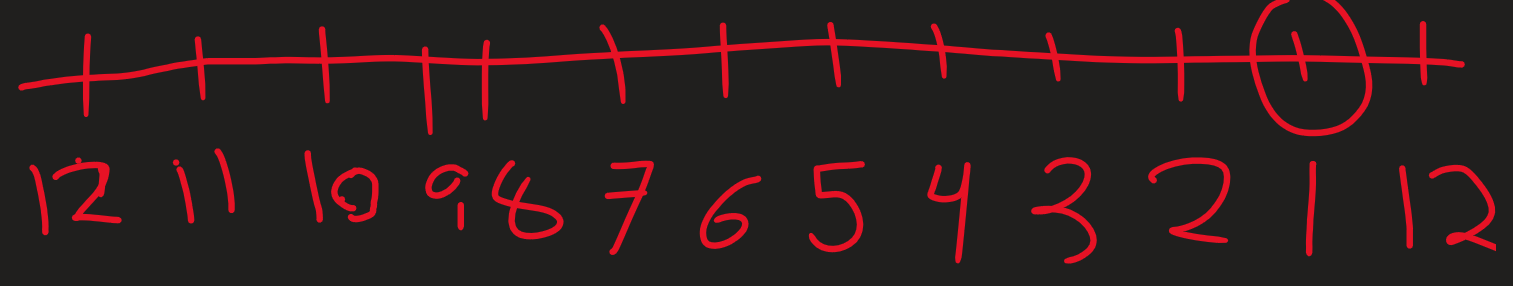
\includegraphics[width=0.5\linewidth]{Images/MarkovProof.png}
                    \caption{Gambling With a Clock}
                \end{figure}
                                
                the probability of reaching 12 on the left is given by $1 - P_{11} = 1 - \frac{11}{12} = \frac{1}{12}$
            \end{solution}
        \end{enumerate}

    \item Before you are six light bulbs (all off), numbered $\{1, 2, \ldots, 6\}$. At each time $n \geq 1$, you roll a fair six-sided die and flip the switch of the bulb corresponding to the number you have rolled, turning it on if it is off, and off if it is on. What is the expected number of rolls needed until every light bulb is turned on?
    

    \item Find the probability that, in the process of repeatedly flipping a fair coin, one will encounter a run of 5 heads in a row before one encounters a run of 2 tails in a row.
    \begin{solution}
        
    \end{solution}

    \item In a game similar to three card monte, the dealer places three cards on the table: the queen of spades and two red cards. The cards are placed in a row, and the queen starts in the center; the card configuration is thus $RQR$. The dealer proceeds to move. With each move, the dealer randomly switches the center card with one of the two edge cards (so the configuration after the first move is either $RRQ$ or $QRR$). What is the probability that, after 2025 moves, the center card is the queen?
\end{enumerate}



\newpage
\subsection{Monday, Apr 14: Problem Session 3}
\begin{enumerate}
\item
Let \(\{X_n\}\) be a Markov chain with state space \(S=\{0,1,2,\ldots\}\). For each of the following transition probabilities, state whether the chain is positive recurrent, null recurrent, or transient. If it is positive recurrent, give the stationary distribution.

\begin{enumerate}[(a)]
    \item \(p(x,x+1)=\frac{5}{7}\), \(p(x,0)=\frac{2}{7}\).
\begin{solution}
    We claim that $\{X_n\}$ is positive recurrent. Indeed, we can see that the stationary distribution must satisfy
    \[\pi_0 = \frac{2}{7}(\sum_{n=0}^\infty \pi_n), \pi_1 = \frac{5}{7}\pi_0, \quad \dots, \pi_n = (\frac{5}{7})^n \pi_0, \quad \sum_{n=0}^\infty \pi_n = 1.\]
    Then 
    \[\pi_n = \left(\frac{5}{7}\right)^n \frac{2}{7}\] is a valid stationary distribution.

\end{solution}
    
    \item \(p(x,0)=\frac{x+1}{x+2}\), \(p(x,x+1)=\frac{1}{x+2}\).
\begin{solution}
    Let $\tau_0 := \{n >0 | X_n = 0 \}.$ Then 
    \[\bbP\{\tau_0  = \infty \mid X_0 = 0\} \geq \prod_{k=1}^\infty \frac{1}{(k+2)} = \lim_{n\to \infty}\frac{1}{(n+2)!} = 0.\] Thus, $\{X_n\}$ is recurrent. Let's check for a stationary distribution!
    
\end{solution}
    \item \(p(x,x+1)=\frac{x+1}{x+2}\), \(p(x,0)=\frac{1}{x+2}\).
    
    \item \(p(x,0)=\frac{1}{x^2+2}\), \(p(x,x+1)=\frac{x^2+1}{x^2+2}\).
\end{enumerate}

\item
Let \(\{X_n\}\) be a biased random walk on \(\mathbb{Z}\) with probability \(p>1/2\) to move to the right, i.e., the transition probabilities are
\[
p(x,x-1)=1-p, \quad p(x,x+1)=p, \quad \forall x\in\mathbb{Z}.
\]
Assume that \(X_0=0\).

\begin{enumerate}[(a)]
    \item Find \(\mathbb{P}[X_n=0]\). \textbf{(Hint:} \(X_n=0\) if and only if we have the same number of \(+1\) steps as \(-1\) steps before time \(n\).)
\begin{solution}
    \[p^{2n}(0,0) = \binom{2n}{n}p^n (1-p)^n\]
\end{solution}
    
    \item For \(K\geq 1\), let \(T_K=\min\{n\geq 1:X_n=K\}\). Find \(\mathbb{P}[X_n\geq 0,\,\forall n=0,\ldots,T_K]\).
\begin{solution}
    This is a shifted gambler's ruin. We can think of it as shifting it by $1$ to the right and the probability of winning $K+1$ dollars before losing it all (starting with one dollar). We have found that 
    \[P_1 = \frac{1 - (\frac{1-p}{p})}{1 - (\frac{1-p}{p})^{K+1}}\]
\end{solution}
    
    \item Find the probability that \(X_n\) returns to 0 after time \(T_K\).
\begin{solution}
    Let $A = \{\exists n >T_K \mid X_n = 0\}.$ Then by the strong Markov property and the law of total probability, if we call
    \[\alpha(k):= \bbP\{A \mid X_0 = k\},\] then
\begin{align*}
   \alpha(k) &= \alpha(k-1)\bbP\{X_1 = K-1\} + \alpha(k+1)\bbP\{X_1 = K+1\}\\
   &= \alpha(k-1)(1-p) + \alpha(k+1)p
\end{align*}
Solving gives 
\[\alpha = \frac{1 \pm \sqrt{1 - 4p(1-p)}}{2p} = \frac{1 \pm (1 - 2p)}{2p} \in \{1, \frac{1-p}{p}\}.\] Thus, 
\[\alpha(n) = \lambda_1 + \lambda_2(\frac{1-p}{p})^n.\] We know that $\alpha(0) = 1.$ Thus, 
\[\lambda_1 + \lambda_2 = 1\] Moreover, we know that 
\[\lim_{n\to \infty}\alpha(n) = 0 = \lambda_1.\] Thus, $\lambda_2 = 1$ and so 
\[\alpha(K) = (\frac{1-p}{p})^K.\]
\end{solution}
    
    \item Find the probability that \(X_n\geq 0\) for all \(n=0,\ldots,T_K\) and \(X_n\) returns to 0 after time \(T_K\).
\begin{solution}
    By the strong Markov Property, these are independent, so simply multiply the results from (ii) and (iii)
\end{solution}
\end{enumerate}

\item
Consider the Markov chain with state space \(\mathbb{Z}\) whose transition probabilities are given by \(p(x,x-1)=2/3\) and \(p(x,x+2)=1/3\) (\(p(x,y)=0\) for all other \(y\)). Determine whether this Markov chain is positive recurrent, null recurrent, or transient. \textbf{(Hint:} use a calculation with the binomial distribution similar to what we did for random walk on \(\mathbb{Z}\).)
\begin{solution}
\begin{align*}
p^{3k}(0,0) &= \binom{3k}{k}(\frac{1}{3})^k(\frac{2}{3})^{2k}\\  &= \frac{(3k)!}{(k)! (2k)!}(\frac{1}{3})^k(\frac{2}{3})^{2k}     \\
&\sim \frac{\sqrt{6\pi k} (\frac{3k}{e})^{3k}}{\sqrt{2\pi k}(\frac{k}{e})^k \sqrt{4\pi k}(\frac{2k}{e})^{2k}}(\frac{1}{3})^k(\frac{2}{3})^{2k} \\
&= \frac{\sqrt{6\pi k} (\frac{3k}{e})^{3k}}{\sqrt{2\pi k}(\frac{k}{e})^k \sqrt{4\pi k}(\frac{2k}{e})^{2k}}(\frac{1}{3})^k(\frac{2}{3})^{2k}\\
&= \sqrt{\frac{3}{4\pi k}}
\end{align*}
We have that 
\[\sum_{k=0}^\infty p^{3k}(0,0)  = \infty,\] and so the process is recurrent. It is null recurrent since $p^n(0,0) \to 0.$

\end{solution}

\item
The \emph{infinite binary tree} is the graph \(T\) whose vertex set \(V(T)\) consists of the empty sequence \(\emptyset\) together with all \(k\)-tuples of the form \((a_1,a_2,\ldots,a_k)\), where \(k\in\mathbb{N}\) and \(a_j\in\{0,1\}\) for \(j\in\{1,\ldots,k\}\). There are edges joining \(\emptyset\) to (0) and (1) and edges joining \((a_1,\ldots,a_k)\) to \((a_1,\ldots,a_k,0)\) and \((a_1,\ldots,a_k,1)\) for each \((a_1,\ldots,a_k)\), see the figure below. Let \(\{X_n\}\) be the random walk on \(T\). Compute
\[
\mathbb{P}[X_n=\emptyset\text{ for some }n\geq 1\,|\,X_0=\emptyset],
\]
and conclude that \(\{X_n\}\) is transient. \textbf{(Hint:} let \(H_n\) be the "height" for \(X_n\), i.e., if \(X_n=\emptyset\) then \(H_n=0\) and if \(X_n=(a_1,\ldots,a_k)\) then \(H_n=k\). Relate \(H_n\) to a biased random walk.)

\end{enumerate}






















\end{document}